%% This file is a portion of the source for Revised Edition 1.1 of
%% Operating Systems and Middleware: Supporting Controlled
%% Interaction, Copyright 2011 by Max Hailperin.  This work is
%% licensed under the Creative Commons Attribution-ShareAlike 3.0
%% Unported License. To view a copy of this license, visit
%% http://creativecommons.org/licenses/by-sa/3.0/ or send a letter to
%% Creative Commons, 171 Second Street, Suite 300, San Francisco,
%% California, 94105, USA.
\chapter{Virtual Memory}\label{vm-chapter}

\section{Introduction}
\label{vm-intro-section}

In Chapters \ref{synchronization-chapter} and \ref{transactions-chapter}, you have seen that synchronization
(including transactions) can control the interactions between
concurrent threads.  For example, synchronization can ensure that only
one thread at a time updates the memory locations holding a shared
data structure.  Now you will learn about another
form of control, which can provide each thread with its own private storage, rather than regulating the threads' access to shared
storage.

In this chapter, I will present a mechanism, \vocab{virtual memory},
that can be used to provide threads with private storage, thereby
controlling their interaction.  However, virtual memory turns out to
be a very general-purpose abstraction, useful for many goals other
than just giving threads some privacy.  Therefore, after using this
introductory section to present the basic concept of virtual memory,
I will devote Section~\ref{vm-uses-section} to surveying the applications of virtual
memory.  Only afterward will I turn to the details of mechanisms and
policies; you'll find the related discussions in Sections \ref{vm-reps} and \ref{vm-policies-section}.  The
chapter concludes with the standard features: security issues in
Section~\ref{vm-security-section}, then exercises, programming and
exploration projects, and notes. 

The essence of virtual memory is to decouple the addresses that
running programs use to identify objects from the addresses that the
memory uses to identify storage locations.  The former are known as
\foldvocabes{virtual}{address} and the latter as \foldvocabes{physical}{address}.  As background for understanding this distinction, consider first
a highly simplified diagram of a computer system, without virtual
memory, as shown in Figure~\ref{PM-diagram}.
\begin{figure}
\centerline{\includegraphics{hail_f0601}}
\iffalse
\centerline{\begin{graph}(252,72)
\graphnodesize{0}
\graphnodecolour{1}
\grapharrowlength{5}
\rectnode{P}[72,72](36,36)
\rectnode{M}[72,72](216,36)
\squarenode{PA}(72,54)
\squarenode{PD}(72,18)
\squarenode{MA}(180,54)
\squarenode{MD}(180,18)
\nodetext{P}{Processor}
\nodetext{M}{Memory}
\diredge{PA}{MA}
\diredge{MD}{PD}
\diredge{PD}{MD}
\bowtext{PA}{MA}{.06}{Address}
\bowtext{PD}{MD}{.06}{Data}
\end{graph}}
\fi
\caption{In a system without virtual memory, the processor sends addresses directly
  to the memory.}
\label{PM-diagram}
\end{figure}
In this system, the processor sends an address to the memory whenever
it wants to store a value into memory or load a value from memory.
The data being loaded or stored is also transferred in the appropriate
direction.  Each load operation retrieves the most recent value stored
with the specified address.  Even though the processor and
memory are using a common set of addresses to communicate, the role
played by addresses is somewhat different from the perspective of the
processor than from the perspective of the memory, as I will now
explain.

From the perspective of the processor (and the program the processor
is executing), addresses are a way of differentiating stored objects
from one another.  If the processor stores more than one value, and
then wishes to retrieve one of those values, it needs to specify which
one should be retrieved.  Hence, it uses addresses essentially as
names.  Just as an executive might tell a clerk to ``file this under
`widget suppliers'\,'' and then later ask the clerk to ``get me that
document we filed under `widget suppliers','' the processor tells the
memory to store a value with a particular address and then later
loads from that address.  Addresses used by executing programs to refer to objects are known as
\foldvocabes{virtual}{address}.

Of course, virtual addresses are not arbitrary names; each virtual address is a
number.  The processor may make use of this to give a group of related
objects related names, so that it can easily compute the name of any
object in the group.  The simplest example of this kind of grouping of
related objects is an array.  All the array elements are stored at
consecutive virtual addresses.  That allows the virtual address of any individual
element to be computed from the base virtual address of the array and the
element's position within the array.

From the memory's perspective, addresses are not identifying names for
objects, but rather are spatial locations of storage cells.  The
memory uses addresses to determine which cells to steer the data into
or out of. Addresses used by the memory
to specify storage locations are known as
\foldvocabes{physical}{address}.  Figure~\ref{scan-6-1} shows the
processor's and memory's views of addresses in a system like
that shown in Figure~\ref{PM-diagram}, where the physical addresses come directly from the virtual addresses, and so are numerically equal.
\begin{figure}
\centerline{\includegraphics{hail_f0602}}
%\centerline{\epsfbox{scan-6-1.eps}}
\caption{In a system without virtual memory, virtual addresses (the
  processor's names for objects) equal physical addresses (the
  memory's storage locations).}
\label{scan-6-1}
\end{figure}

The difference between the processor's and memory's perspectives becomes apparent when you consider that
the processor may be dividing its time between multiple computational
processes.
Sometimes the processes will each need a private object,
yet the natural name to use will be the same in more than one process.
Figure~\ref{scan-6-2} shows how this necessitates using different
addresses in the processor and the memory.  That is, virtual addresses
can no longer be equal to physical addresses.
\begin{figure}
\centerline{\includegraphics{hail_f0603}}
%\centerline{\epsfbox{scan-6-2.eps}}
\caption{When two processes each use the same virtual
  addresses as names for their own objects, the virtual addresses
  cannot equal the physical addresses, because each process's objects
  need to be stored separately.}
\label{scan-6-2}
\end{figure}
To make this work, general-purpose computers are
structured as shown in Figure~\ref{PMM-diagram}.
\begin{figure}
\centerline{\includegraphics{hail_f0604}}
\iffalse
\centerline{\begin{graph}(312,83)
\graphnodesize{0}
\graphnodecolour{1}
\grapharrowlength{5}
\rectnode{P}[72,72](36,36)
\rectnode{M}[72,72](276,36)
\rectnode{MMU}[36,36](156,54)
\squarenode{PA}(72,54)
\squarenode{PD}(72,18)
\squarenode{MA}(240,54)
\squarenode{MD}(240,18)
\squarenode{MMUV}(138,54)
\squarenode{MMUP}(174,54)
\nodetext{P}{Processor}
\nodetext{M}{Memory}
\nodetext{MMU}{MMU}
\diredge{PA}{MMUV}
\diredge{MMUP}{MA}
\diredge{MD}{PD}
\diredge{PD}{MD}
\bowtext{PA}{MMUV}{.22}{\begin{tabular}{c}Virtual\\address\end{tabular}}
\bowtext{MMUP}{MA}{.22}{\begin{tabular}{c}Physical\\address\end{tabular}}
\bowtext{PD}{MD}{.04}{data}
\end{graph}}
\fi
\caption{The memory management unit (MMU) translates the processor's virtual
  addresses into the memory's physical addresses.}
\label{PMM-diagram}
\end{figure}
Program execution within the processor works entirely in terms of
virtual addresses.  However, when a load or store operation is
executed, the processor sends the virtual address to an intermediary,
the \vocab{memory management unit} (\vocab{MMU}).  The MMU translates
the virtual address into a corresponding physical address, which it
sends to the memory.

In Figure~\ref{scan-6-2}, each process uses the virtual address 0 as a
name for its own triangle.  This is a simplified model of how more complicated
objects are referenced by real processes.
Consider next a more realistic example of why each process might use the same
virtual addresses for its own objects.  Suppose several copies of the
same spreadsheet program are running.  Each copy will naturally want
to refer to ``the spreadsheet,'' but it should be a different
spreadsheet object in each process.  Even if each process uses a numerical name
(that is, a virtual address), it would be natural for all running instances of
the spreadsheet program to use the same address; after all, they are
running the same code.  Yet from the memory's perspective, the
different processes' objects need to be stored separately---hence, at
different physical addresses.

The same need for private names arises, if not quite so strongly, even
if the concurrent processes are running different programs.  Although in
principle each application program could use different names (that is,
virtual addresses) from all other programs, this requires a rather unwieldy
amount of coordination.

Even for shared objects, addresses as names behave somewhat
differently from addresses as locations.  Suppose two processes are
communicating via a shared bounded buffer; one is the producer, while
the other is the consumer.  From the perspective of one process, the
buffer is the ``output channel,'' whereas for the other process, it is
the ``input channel.''  Each process may have its own name for the
object; yet, the memory still needs to store the object in one location.
This holds true as well if the names used by the processes are numerical
virtual addresses.

Thus, once again, virtual addresses and physical
addresses should not be forced to be equal; it should be possible for
two processes to use the same virtual address to refer to different
physical addresses or to use different virtual addresses to refer to the
same physical address.

You have seen that the MMU maps virtual addresses to physical
addresses.  However, I have not yet discussed the nature of this mapping.  So
far as anything up to this point goes, the mapping could be as
simple as computing each physical address as twice the virtual
address.  However, that would not yield the very general mechanism
known as virtual memory.  Instead, virtual memory must have the following
additional properties:
\begin{itemize}
\item
The function that maps virtual addresses to physical addresses is
represented by a table, rather than by a computational rule (such as
doubling).  That way, the mapping can be much more general.
\item
However, to keep its size manageable, the table does not independently
list a physical address for each virtual address.  Instead, the
virtual addresses are grouped together into blocks known as
\vocabs{page}, and the table shows for each page of virtual addresses
the corresponding \vocab{page frame} of physical addresses.  I'll explain
this in greater detail in Section~\ref{vm-reps}.
In that same section, I also briefly
consider an alternative, \vocab{segmentation}.
\item
The contents of the table are controlled by the operating system.
This includes both incremental adjustments to the table (for purposes
you will see in Section~\ref{vm-uses-section}) and wholesale changes of the table
when switching between threads.  The latter allows each thread to have
its own private virtual address space, in which case, the threads belong to
different processes, as explained in Section~\ref{vm-private-storage-section}.
\item
The table need not contain a physical address translation for every
page of virtual addresses; in effect, some entries can be left blank.
These undefined virtual addresses are illegal for the processor to
use.  If the processor generates an illegal address, the MMU
interrupts the processor, transferring control to the operating
system.  This interrupt is known as a \vocab{page fault}.  This
mechanism serves not only to limit the usable addresses but also to
allow address translations to be inserted into the table only when
needed.  By creating address translations in this demand-driven fashion, many applications of virtual memory arrange to move data only when necessary,
thereby improving performance.
\item
As a refinement of the notion of illegal addresses, some entries in
the table may be marked as legal for use, but only in specific ways.  Most
commonly, it may be legal to read from some particular page of virtual
addresses but not to write into that page.  The main purpose this
serves is to allow trouble-free sharing of memory between processes.
\end{itemize}

In summary, then, virtual memory consists of an
operating system--defined table of mappings from virtual addresses to
physical addresses (at the granularity of pages), with the opportunity
for intervention by the operating system on accesses that the table
shows to be illegal.  You should be able to see that this is a very
flexible mechanism.  The operating system can switch between multiple
views of the physical memory.  Parts of physical memory may be
completely invisible in some views, because no virtual addresses map
to those physical addresses.  Other parts may be visible in more than
one view, but appearing at different virtual addresses.  Moreover, the
mappings between virtual and physical addresses need not be
established in advance.  By marking pages as illegal to access, and
then making them available when an interrupt indicates that they are
first accessed, the operating system can provide mappings on a
demand-driven basis.  In Section~\ref{vm-uses-section}, you will see several
uses to which this general mechanism can be put.

\section{Uses for Virtual Memory}\label{vm-uses-section}

This section contains a catalog of uses for virtual memory, one per subsection.
The applications of virtual memory enumerated are all
in everyday use in most general-purpose operating systems.  A
comprehensive list would be much longer and would include some
applications that have thus far been limited to research systems or
other esoteric settings.

\subsection{Private Storage}\label{vm-private-storage-section}

The introductory section of this chapter has already explained that each computation
running on a computer may want to have its own private storage,
independent of the other computations that happen to be running on the
same computer.  This goal of private storage can be further elaborated
into two subgoals:
\begin{itemize}
\item
Each computation should be able to use whatever virtual addresses it
finds most convenient for its objects, without needing to avoid using
the same address as some other computation.
\item
Each computation's objects should be protected from accidental (or
malicious) access by other computations.
\end{itemize}
Both subgoals---independent allocation and protection---can be
achieved by giving the computations their own virtual memory
mappings.  This forms the core of the process concept.

A \vocab{process} is a group of one or more threads with an associated
protection context.  I will introduce processes more fully in
Chapter~\ref{processes-chapter}.  In
particular, you will learn that the phrase ``protection context'' is
intentionally broad, including such protection features as file access permissions,
which you will study in Chapters \ref{processes-chapter} and \ref{persistence-chapter}.  For now, I will focus on
one particularly important part of a process's context: the mapping
of virtual addresses to physical addresses.  In other words, for the
purposes of this chapter, a process is a group of threads that share a virtual
address space.

As I will describe in Chapter~\ref{processes-chapter}, the computer hardware and
operating system software collaborate to achieve protection by
preventing any software outside the operating system from updating the
MMU's address mapping.  Thus, each process is restricted to accessing
only those physical memory locations that the operating system
has allocated as page frames for that process's pages.  Assuming that
the operating system allocates different processes disjoint portions
of physical memory, the processes will have no ability to interfere with one
another.  The physical memory areas for the processes need only
be disjoint at each moment in time; the processes can take
turns using the same physical memory.

This protection model, in which processes are given separate virtual
address spaces, is the mainstream approach today; for the purposes of
the present chapter, I will take it for granted.  In Chapter~\ref{processes-chapter}, I will also explore alternatives that allow all processes to
share a single address space and yet remain protected from one
another.

\subsection{Controlled Sharing}
\label{controlled-sharing-subsection}
Although the norm is for processes to use disjoint storage, sometimes
the operating system will map a limited portion of memory into more
than one process's address space.  This limited sharing may be a way
for the processes to communicate, or it may simply be a way to reduce
memory consumption and the time needed to initialize memory.  Regardless of the motivation, the shared physical
memory can occupy a different range of virtual addresses in each
process.  (If this flexibility is exercised, the shared memory should
not be used to store pointer-based structures, such as linked lists,
because pointers are represented as virtual addresses.)

The simplest example of memory-conserving sharing occurs when multiple
processes are running the same program.  Normally, each process divides
its virtual address space into two regions:
\begin{itemize}
\item
A read-only region holds the machine language instructions of the
program, as well as any read-only data the program contains, such as
the character strings printed for error messages.  This region is
conventionally called the \vocab{text} of the program.
\item
A read/write region holds the rest of the process's data.  (Many
systems actually use two read/write regions, one for the stack and one
for other data.)
\end{itemize}
All processes running the same program can share the same text.  The
operating system maps the text into each process's virtual memory address
space, with the protection bits in the MMU set to enforce read-only
access.  That way, the shared text does not accidentally become a
communication channel.

Modern programs make use of large libraries of supporting
code.  For example, there is a great deal of code related to graphical
user interfaces that can be shared among quite different programs,
such as a web browser and a spreadsheet.  Therefore, operating systems
allow processes to share these libraries with read-only protection,
just as for main programs.  Microsoft refers to shared libraries as
\vocabyies{dynamic-link librar} (\vocabs{DLL}).

Figure~\ref{scan-6-3} illustrates how processes can share in read-only
form both program text and the text of DLLs.  In this figure,
processes A and B are running program 1, which uses DLLs 1 and 2.
Processes C and D are running program 2, which uses DLLs 1 and 3.
Each process is shown as encompassing the appropriate program text,
DLLs, and writable data area.  In other words, each process encompasses
those areas mapped into its virtual address space.
\begin{figure}
\centerline{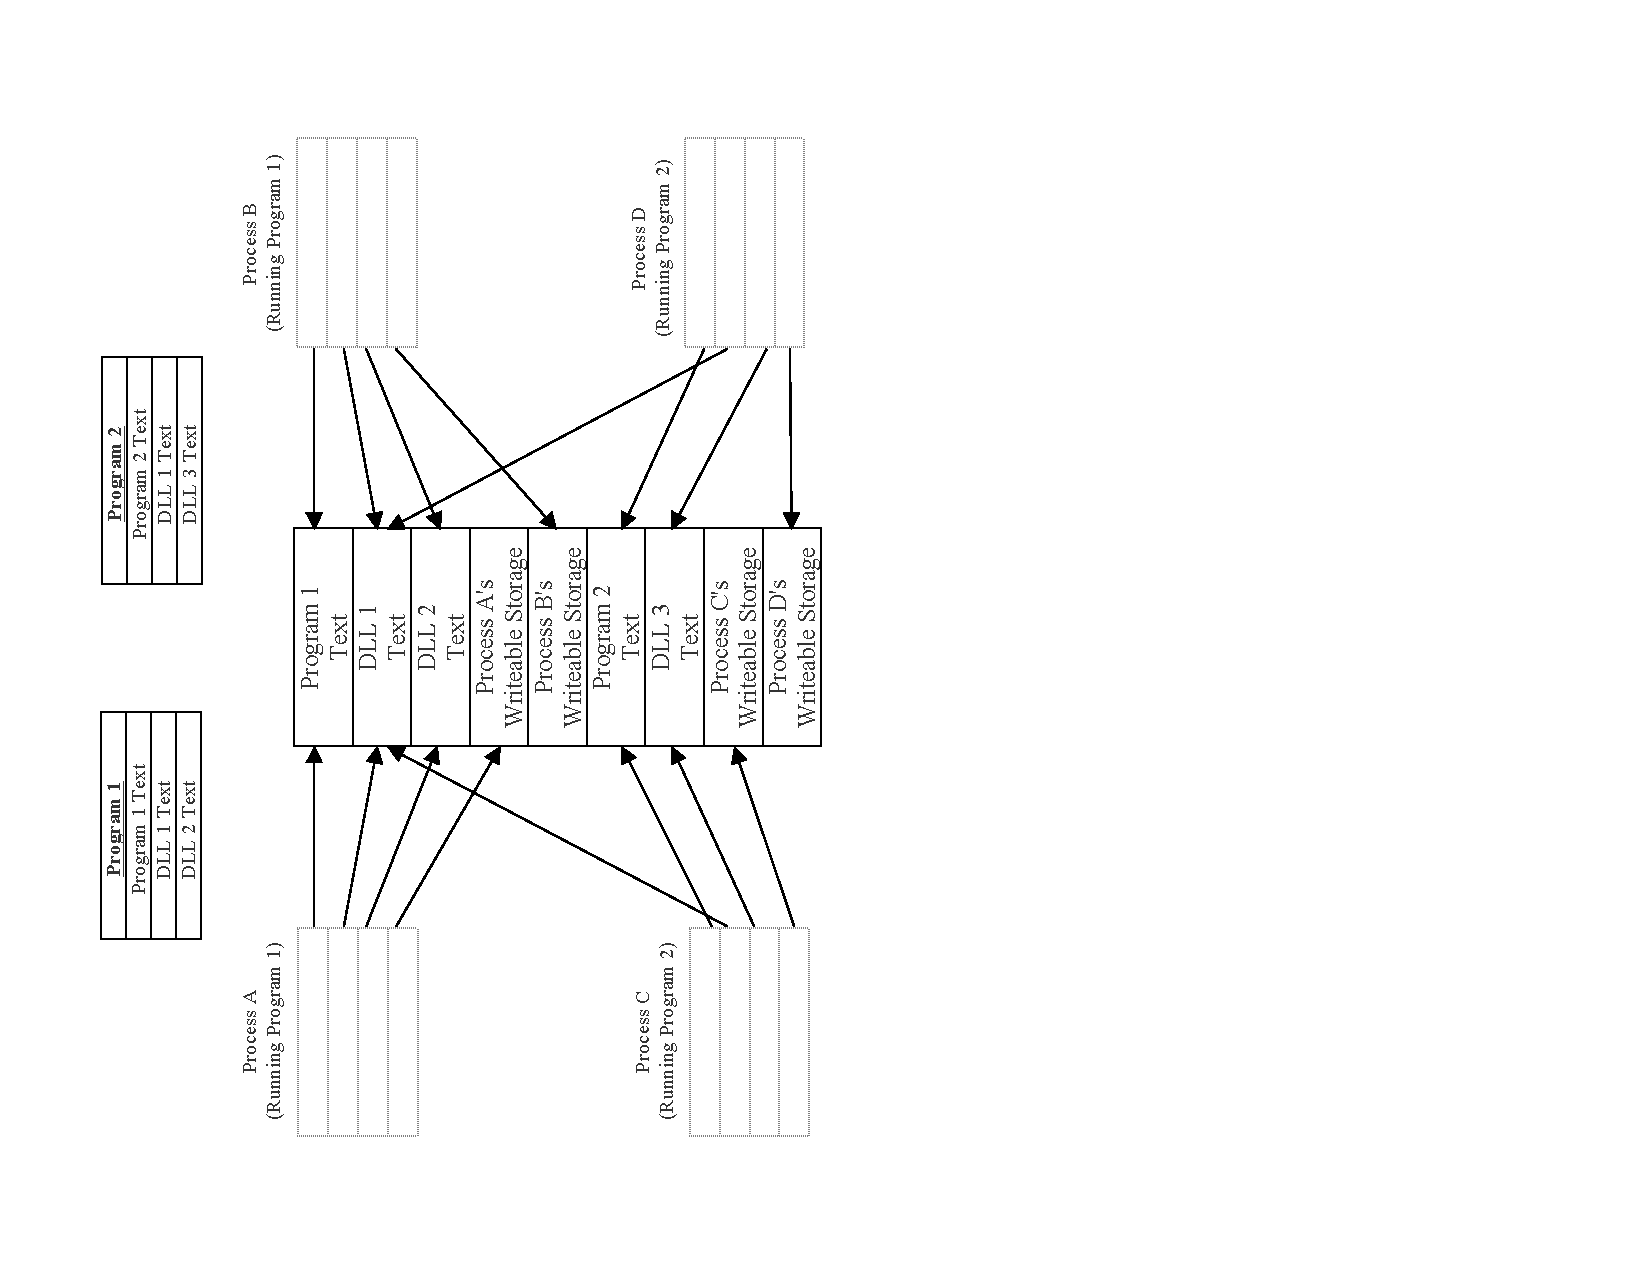
\includegraphics{hail_f0605}}
%\centerline{\epsfbox{scan-6-3.eps}}
\caption{The address space of a process includes the text of the
  program the process is running, the text of any DLLs used by that
  program, and a writable storage area for data.  Because processes A and B are
  both running program 1, which uses DLLs 1 and 2, their address
  spaces share these components.  Processes C and D are running
  program 2, which uses DLLs 1 and 3.  Because both programs use
  DLL~1, all four processes share it.}
\label{scan-6-3}
\end{figure}


From the operating system's perspective, the simplest way to support
interprocess communication is to map some physical memory into two
processes' virtual address spaces with full read/write permissions.
Then the processes can communicate freely; each
writes into the shared memory and reads what the other one writes.
Figure~\ref{scan-6-4} illustrates this sharing of a writable
area of memory for communication.
\begin{figure}
\centerline{\includegraphics{hail_f0606}}
%\centerline{\epsfbox{scan-6-4.eps}}
\caption{Two processes can communicate by sharing a writable storage area.}
\label{scan-6-4}
\end{figure}

Simple as this may be for the operating system, it is anything but
simple for the application programmers.  They need to include mutexes,
readers-writers locks, or some similar synchronization structure in
the shared memory, and they need to take scrupulous care to use those
locks.  Otherwise, the communicating processes will exhibit races,
which are difficult to debug.

Therefore, some operating systems (such as Mac OS~X) use virtual
memory to support a more structured form of communication, known as
\vocab{message passing}, in which
one process writes a message into a block of memory and then asks the
operating system to send the message to the other process.  The
receiving process seems to get a copy of the sent message.  For small
messages, the operating system may literally copy the message from one
process's memory to the other's.  For efficiency, though, large
messages are not actually copied.  Instead, the operating system
updates the receiver's virtual memory map to point at the same
physical memory as the sender's message; thus, sender and receiver
both have access to the message, without it being copied.  To maintain
the ease of debugging that comes from message passing, the operating
system marks the page as read-only for both the sender and the
receiver.  Thus, they cannot engage in any nasty races.  Because the
sender composes the message before invoking the operating system, the
read-only protection is not yet in place during message composition
and so does not stand in the way.

As a final refinement to message passing by read-only sharing, systems
such as Mac OS~X offer \vocab{copy on write} (\vocab{COW}).  If either
process tries to write into the shared page, the MMU will use an
interrupt to transfer control to the operating system.  The operating
system can then make a copy of the page, so that the sender and
receiver now have their own individual copies, which can be
writable.  The operating system resumes the process that was trying
to write, allowing it to now succeed.  This provides the complete
illusion that the page was copied at the time the message was sent, as
shown in Figure~\ref{scan-6-5}.
\begin{figure}
\centerline{\includegraphics{hail_f0607}}
%\centerline{\epsfbox{scan-6-5.eps}}
\caption{To use copy on write (COW) message passing, process~A
  writes a message into part of its private memory (Step~1) and then
  asks the operating system to map the memory containing the message into process~B's
  address space as well (Step~2).  Neither process has permission to write into
  the shared area.  If either violates this restriction, the operating
  system copies the affected page, gives each process write
  permission for its own copy, and allows the write operation to
  proceed (Step~3).  The net effect is the same as if the message were copied
  when it was sent, but the copying is avoided if neither process writes into
  the shared area.}
\label{scan-6-5}
\end{figure}
The advantage is that if the processes do not write into most message pages, most
of the copying is avoided.

\subsection{Flexible Memory Allocation}

The operating system needs to divide the computer's memory among
the various processes, as well as retain some for its own use.
At first glance, this memory allocation problem doesn't seem too
difficult.  If one process needs 8 megabytes (MB) and another needs
10, the operating system could allocate the first 8~MB of
the memory (with the lowest physical addresses) to the first process
and the next 10~MB to the second.  However, this kind of
contiguous allocation runs into two difficulties.

The first problem with contiguous allocation is that the amount of
memory that each process requires may grow and shrink as the program
runs.  If the first process is immediately followed in memory by the
second process, what happens if the first process needs more space?

The second problem with contiguous allocation is that processes exit,
and new processes (with different sizes) are started.  Suppose you have
512~MB of memory available and three processes running, of sizes
128~MB, 256~MB, and 128~MB.  Now suppose the first and third processes
terminate, freeing up their 128-MB chunks of memory.  Suppose a 256-MB
process now starts running.  There is enough memory available, but not
all in one contiguous chunk, as illustrated in Figure~\ref{scan-6-6}.
\begin{figure}
\centerline{\includegraphics{hail_f0608}}
%\centerline{\epsfbox{scan-6-6.eps}}
\caption{Contiguous allocation leads to external fragmentation.  In
  this example, there is no contiguous 256-MB space available for
  process~D, even though the termination of processes A and C has
  freed up a total of 256~MB.}
\label{scan-6-6}
\end{figure}
This situation is known as \foldvocab{external}{fragmentation}.  I
will discuss external fragmentation more carefully in
Chapter~\ref{persistence-chapter}, because contiguous allocation is
important for disk space.  (I will also define the contrasting term,
internal fragmentation, in that same chapter.)

Because all modern general-purpose systems have virtual memory, these
contiguous allocation difficulties are a non-issue for main memory.
The operating system can allocate any available physical page frames
to a process, independent of where they are located in memory. 
For example, the conundrum of
Figure~\ref{scan-6-6} could be solved as shown in
Figure~\ref{discontiguous}.
\begin{figure}
\centerline{\includegraphics{hail_f0609}}
%\centerline{\epsfbox{discontiguous.eps}}
\caption{With virtual memory, the physical memory allocated to a
  process need not be contiguous, so process~D can be accommodated even
  without sufficient memory in any one place.}
\label{discontiguous}
\end{figure}
In a more realistic setting, it would be
surprising for the pattern of physical memory allocation to display
even this degree of contiguity.  However, the
virtual addresses can be contiguous even if the physical addresses
are scattered all over the memory. 

\subsection{Sparse Address Spaces}

Just as virtual memory provides the operating system with flexibility
in allocating physical memory space, it provides each application
program (or process) with flexibility in allocating virtual address
space.  A process can use whatever addresses make sense for its data
structures, even if there are large gaps between them.  This provides
flexibility for the compiler and runtime environment, which assign
addresses to the data structures.

Suppose, for example, that a process has three data structures (S1, S2, and
S3) that it needs to store.  Each needs to be allocated in a
contiguous range of addresses, and each needs to be able to grow at
its upper end.  The picture might look like this, with addresses in megabytes:
\[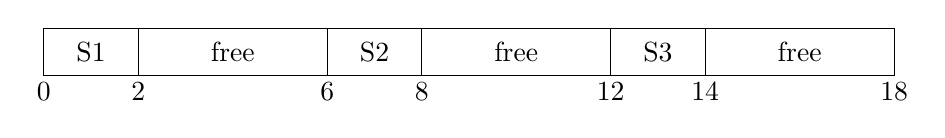
\begin{tikzpicture}[scale=.03]
\draw (0,0) rectangle (40,20);
\draw (40,0) rectangle (120,20);
\draw (120,0) rectangle (160,20);
\draw (160,0) rectangle (240,20);
\draw (240,0) rectangle (280,20);
\draw (280,0) rectangle (360,20);
\draw (20,10) node{S1};
\draw (80,10) node{free};
\draw (140,10) node{S2};
\draw (200,10) node{free};
\draw (260,10) node{S3};
\draw (320,10) node{free};
\draw (0,-7) node{0};
\draw (40,-7) node{2};
\draw (120,-7) node{6};
\draw (160,-7) node{8};
\draw (240,-7) node{12};
\draw (280,-7) node{14};
\draw (360,-7) node{18};
\end{tikzpicture}\]
\iffalse
\[\begin{graph}(370,32)(-3,-12)
\graphlinecolour{0}
\fillednodesfalse
\rectnode{a}[40,20](20,10)
\rectnode{b}[80,20](80,10)
\rectnode{c}[40,20](140,10)
\rectnode{d}[80,20](200,10)
\rectnode{e}[40,20](260,10)
\rectnode{f}[80,20](320,10)
\autonodetext{a}{S1}
\autonodetext{b}{free}
\autonodetext{c}{S2}
\autonodetext{d}{free}
\autonodetext{e}{S3}
\autonodetext{f}{free}
\freetext(0,-7){0}
\freetext(40,-7){2}
\freetext(120,-7){6}
\freetext(160,-7){8}
\freetext(240,-7){12}
\freetext(280,-7){14}
\freetext(360,-7){18}
\end{graph}\]
\fi
In this example, only one third of the 18-MB address range is actually
occupied.  If you wanted to allow each structure to grow more, you would
have to position them further apart and wind up with an even lower
percentage of occupancy.  Many real processes span an address range of
several gigabytes without using anywhere near that much storage.
(Typically, this is done to allow one region to grow up from the
bottom of the address space and another to grow down from the top.)

In order to allow processes to use this kind of
\foldvocab{sparse}{address space} without wastefully occupying a
corresponding amount of physical memory, the operating system simply
doesn't provide physical address mappings for virtual addresses in the
gaps.

\subsection{Persistence}

Any general-purpose operating system must provide some way for users
to retain important data even if the system is shut down and
restarted.  Most commonly, the data is kept in files, although other
kinds of persistent objects can be used.  The persistent objects are
normally stored on disk. For example, as I write this book, I am
storing it in files on disk.  That way, I don't have to retype the
whole book every time the computer is rebooted.  I will consider
persistence in more detail in Chapter~\ref{persistence-chapter}; for
now, the only question is how it relates to virtual memory.

When a process needs to access a file (or other persistent object),
it can ask the operating system to map the file into its address
space.  The operating system doesn't actually have to read the whole
file into memory.  Instead, it can do the reading on a demand-driven
basis.  Whenever the process accesses a particular page of the file
for the first time, the MMU signals a page fault.  The operating
system can respond by reading that page of the file into memory,
updating the mapping information, and resuming the process. (For
efficiency reasons, the operating system might choose to fetch
additional pages at the same time, on the assumption they are likely
to be needed soon.  I discuss this possibility in Section~\ref{fetch-policy}.)

If the process writes into any page that
is part of a mapped file, the operating system must remember to write
the page back to disk, in order to achieve persistence.  For efficiency, the
operating system should not write back pages that have not been
modified since they were last written back or since they were read in.
This implies the operating system needs to know which pages have been
modified and hence are not up to date on disk.  (These are called
\vocab{dirty} pages.)

One way to keep track of dirty pages, using only techniques I have
already discussed, is by initially marking all pages read-only.  That
way, the MMU will generate an interrupt on the first attempt to write
into a clean page.  The operating system can then make the page
writable, add it to a list of dirty pages, and allow the operation to
continue.  When the operating system makes the page clean again, by
writing it to disk, it can again mark the page read-only.

Because keeping track of dirty pages is such a common requirement and
would be rather inefficient using the approach just described, MMUs
generally provide a more direct approach.  In this approach, the MMU keeps a
\vocab{dirty bit} for each page.  Any write into the page causes the
hardware to set the dirty bit without needing operating system
intervention.  The operating system can later read the dirty bits and
reset them.  (The Intel Itanium architecture contains a compromise:
the operating system sets the dirty bits, but with some hardware
support.  This provides the flexibility of the software approach
without incurring so large a performance cost.)

\subsection{Demand-Driven Program Loading}

One particularly important case in which a file gets mapped into memory is
running a program.  Each executable program is ordinarily stored as a
file on disk.  Conceptually, running a program consists of reading the
program into memory from disk and then jumping to the first
instruction.

However, many programs are huge and contain parts that may not always
be used.  For example, error handling routines will get used only if
the corresponding errors occur.  In addition, programs often support more
features and optional modes than any one user will ever need.  Thus,
reading in the whole program is quite inefficient.

Even in the rare case that the whole program gets used, an interactive
user might prefer several short pauses for disk access to one long
one.  In particular, reading in the whole program initially means that
the program will be slow to start, which is frustrating.  By reading
in the program incrementally, the operating system can start it
quickly at the expense of brief pauses during operation.  If each of
those pauses is only a few tens of milliseconds in duration and
occurs at the time of a user interaction, each will be below the
threshold of human perception.

In summary, operating system designers have two reasons to use virtual memory
techniques to read in each program on a demand-driven basis: in order to avoid
reading unused portions and in order to quickly start the program's execution.  As with more general
persistent storage, each page fault causes the operating system to
read in more of the program.

One result of demand-driven program loading is that application programmers can make their
programs start up more quickly by grouping all the necessary code together
on a few pages. Of
course, laying out the program text is really not a job for the
human application programmer, but for the compiler and linker.
Nonetheless, the programmer may be able to provide some guidance to these tools.

\subsection{Efficient Zero Filling}

For security reasons, as well as for ease of debugging, the operating
system should never let a process read from any memory location that
contains a value left behind by some other process that previously
used the memory.  Thus, any memory not occupied by a persistent
object should be cleared out by the operating system before a new process accesses it.

Even this seemingly mundane job---filling a region of memory with
zeros---benefits from virtual memory.  The operating system can fill
an arbitrarily large amount of virtual address space with zeros using
only a single zeroed-out page frame of physical memory.  All it needs
to do is map all the virtual pages to the same physical page frame
and mark them as read-only.

In itself, this technique of sharing a page frame of zeros
doesn't address the situation where a process writes into one of its
zeroed pages.  However, that situation can be handled using a variant of the COW technique
mentioned in Section~\ref{controlled-sharing-subsection}.  When the MMU
interrupts the processor due to a write into the read-only page of
zeros, the operating system can update the mapping for that one page
to refer to a separate read/write page frame of zeros and then resume the
process.

If it followed the COW principle literally, the operating system would
copy the read-only page frame of zeros to produce the separate,
writable page frame of zeros.  However, the operating system can run faster
by directly writing zeros into the new page frame without needing to
copy them out of the read-only page frame. In fact, there is no
need to do the zero filling only on demand.  Instead, the operating
system can keep some spare page frames of zeros around, replenishing
the stock during idle time.  That way, when a page fault occurs from
writing into a read-only page of zeros, the operating system can simply
adjust the address map to refer to one of the spare prezeroed page
frames and then make it writable.

When the operating system proactively fills spare page frames with zeros
during idle time, it should bypass the processor's normal cache memory
and write directly into main memory.  Otherwise, zero filling can
seriously hurt performance by displacing valuable data from the cache.

\subsection{Substituting Disk Storage for RAM}
\label{disk-for-RAM}
In explaining the application of virtual memory to persistence, I
showed that the operating system can read accessed pages into memory
from disk and can write dirty pages back out to disk.  The reason for
doing so is that disk storage has different properties from main
semiconductor memory (RAM).  In the case of persistence, the relevant
difference is that disk storage is nonvolatile; that is, it retains its
contents without power.  However, disk differs from RAM in other
regards as well.  In particular, it is a couple orders of magnitude
cheaper per gigabyte.  This motivates another use of virtual memory,
where the goal is to simulate having lots of RAM using less-expensive
disk space.  Of course, disk is also five orders of magnitude slower
than RAM, so this approach is not without its pitfalls.

Many processes have long periods when they are not actively running.
For example, on a desktop system, a user may have several applications
in different windows---a word processor, a web browser, a mail reader,
a spreadsheet---but focus attention on only one of them for minutes or
hours at a time, leaving the others idle.  Similarly, within a
process, there may be parts that remain inactive.  A spreadsheet user
might look at the online help once, and then not again during several
days of spreadsheet use.

This phenomenon of inactivity provides an opportunity to capitalize on
inexpensive disk storage while still retaining most of the
performance of fast semiconductor memory.  The computer system needs
to have enough RAM to hold the \vocab{working set}---the active
portions of all active processes.  Otherwise, the performance will be
intolerably slow, because of disk accesses made on a routine basis.  However,
the computer need not have enough RAM for the entire storage needs of
all the processes: the inactive portions can be shuffled off to disk,
to be paged back in when and if they again become active.  This will
incur some delays for disk access when the mix of activity changes,
such as when a user sets the word processor aside and uses a spreadsheet
for the first time in days.  However, once the new working set of
active pages is back in RAM, the computer will again be as responsive
as ever.

Much of the history of virtual memory focuses on this one application,
dating back to the invention of virtual memory in the early 1960s.
(At that time, the two memories were magnetic cores and magnetic drum,
rather than semiconductor RAM and magnetic disk.)  Even though this
kind of paging to disk has become only one of many roles played by
virtual memory, I will still pay it considerable attention.  In particular,
some of the most interesting policy questions arise only for this
application of virtual memory.  When the operating system needs to
free up space in overcrowded RAM, it needs to guess which pages are
unlikely to be accessed soon. I will come back to this topic
(so-called replacement policies) after first considering other
questions of mechanism and policy that apply across the full spectrum
of virtual memory applications.

\section{Mechanisms for Virtual Memory}
\label{vm-reps}

Address mapping needs to be flexible, yet efficient. As I mentioned
in Section~\ref{vm-intro-section}, this means that the mapping function is stored in an explicit
table, but at the granularity of pages rather than individual bytes or
words.  Many systems today use fixed-size pages, perhaps with a few
exceptions for the operating system itself or hardware access, though
research suggests that more general mixing of page sizes can be
beneficial.  (As explained in the notes, Linux has moved in this direction.)

Typical page sizes have grown over the decades, for reasons you can
explore in Exercises \ref{page-size-execercise-1} and \ref{page-size-execercise-2}; today, the most common
is 4 kilobytes (KB).  Each page of virtual memory and each page frame of physical
memory is this size, and each starts at an address that is a multiple
of the page size.  For example, with 4-KB pages, the first page (or
page frame) has address 0, the next has address 4096, then 8192, and
so forth.

Each page of virtual memory address space maps to an underlying page
frame of physical memory or to none. For example,
Figure~\ref{example-mapping} shows one possible mapping, on a system
with unrealistically few pages and page frames.
\begin{figure}
\centerline{\includegraphics{hail_f0610}}
\iffalse
\centerline{\begin{graph}(100,200)
\graphlinecolour{0}
\grapharrowlength{5}
\fillednodesfalse
\graphnodesize{20}
\squarenode{p0}(20,150)
\squarenode{p1}(20,130)
\squarenode{p2}(20,110)
\squarenode{p3}(20,90)
\squarenode{p4}(20,70)
\squarenode{p5}(20,50)
\squarenode{p6}(20,30)
\squarenode{p7}(20,10)
\squarenode{f0}(100,110)
\squarenode{f1}(100,90)
\squarenode{f2}(100,70)
\squarenode{f3}(100,50)
\textnode{x2}(50,110){X}[\graphlinewidth{0}\graphlinecolour{1}]
\textnode{x3}(50,90){X}[\graphlinewidth{0}\graphlinecolour{1}]
\textnode{x4}(50,70){X}[\graphlinewidth{0}\graphlinecolour{1}]
\textnode{x5}(50,50){X}[\graphlinewidth{0}\graphlinecolour{1}]
\textnode{x7}(50,10){X}[\graphlinewidth{0}\graphlinecolour{1}]
\autonodetext{p0}[w]{0}
\autonodetext{p1}[w]{1}
\autonodetext{p2}[w]{2}
\autonodetext{p3}[w]{3}
\autonodetext{p4}[w]{4}
\autonodetext{p5}[w]{5}
\autonodetext{p6}[w]{6}
\autonodetext{p7}[w]{7}
\autonodetext{f0}[e]{0}
\autonodetext{f1}[e]{1}
\autonodetext{f2}[e]{2}
\autonodetext{f3}[e]{3}
\diredge{p0}{f1}
\diredge{p1}{f0}
\diredge{p2}{x2}
\diredge{p3}{x3}
\diredge{p4}{x4}
\diredge{p5}{x5}
\diredge{p6}{f3}
\diredge{p7}{x7}
\freetext(20,170){Pages}
\freetext(100,130){Page frames}
\end{graph}}
\fi
\caption{In this example mapping of eight pages to four page frames,
  page~0 has been allocated page frame~1, page~1 has been allocated
  page frame~0, and page~6 has been allocated page frame~3.  The Xs
  indicate that no page frame is assigned to hold pages 2--5 or
  page 7.  Page frame~2 is unused.}
\label{example-mapping}
\end{figure}
The numbers next to the
boxes are page numbers and page frame numbers.  The starting
addresses are these numbers multiplied by the page size.
At the top of this figure, you can see that page~0 is stored in page
frame~1.  If the page size is 4~KB, this means that virtual address 0
translates to physical address 4096, virtual address 100 translates to
physical address 4196, and so forth.  The virtual address of the last
4-byte word in
page~0, 4092, translates to the physical address of the last word in page frame~1,
8188.  Up until this point, all physical addresses were found by
adding 4096 to the virtual address.  However, the very next virtual
address, 4096, translates to physical address 0, because it starts a
new page, which is mapped differently.  Note also that page frame~2 is
currently not holding any page, and that pages 2--5 and page~7 have no
translation available.  In
Exercise~\ref{page-6-translation-exercise}, you can gain experience working with this
translation of virtual addresses into physical addresses by
translating the addresses for page~6.

Of course, a realistic computer system will have many more page frames
of physical memory and pages of virtual address space.  Often there
are tens or hundreds of thousands of page frames and at least
hundreds of thousands of pages.  As a result, operating system
designers need to think carefully about the data structure used to
store the table that maps virtual page numbers to physical page frame
numbers.  Sections \ref{linear-page-tables-section} through \ref{hashed-page-tables-section} will be devoted to presenting three
alternative structures that are in current use for page tables:
linear, multilevel, and hashed.  (Other alternatives that have fallen
out of favor, or have not yet been deployed, are briefly mentioned in
the end-of-chapter notes.)

Whatever data structure the operating system uses for its page table,
it will need to communicate the mapping information to the hardware's
MMU, which actually performs the mapping.  The nature of this
software/hardware interface constrains the page table design and also
provides important context for comparing the performance of
alternative page table structures.  Therefore, in
Section~\ref{vm-hw-sw-interface}, I will explain the two
forms the software/hardware interface can take.

Finally, Section~\ref{vm-segmentation-section} provides a brief look at segmentation, which was
historically important both as an alternative to paging and as an
adjunct to it.

\subsection{Software/Hardware Interface}\label{vm-hw-sw-interface}

You have seen that the operating system stores some form of page table
data structure in memory, showing which physical memory page frame (if
any) holds each virtual memory page.  Although I will present
several possible page table structures shortly, the most important
design issue applies equally to all of them: the page table should
almost never be used.

Performance considerations explain why such an important data
structure should be nearly useless (in the literal sense).  Every
single memory access performed by the processor generates a virtual
address that needs translation to a physical address.  Naively, this
would mean that every single memory access from the processor requires
a lookup operation in the page table.  Performing that lookup
operation would require at least one more memory access, even if the
page table were represented very efficiently.  Thus, the number of
memory accesses would at least double: for each real access, there
would be one page table access.  Because memory performance is often the
bottleneck in modern computer systems, this means that virtual memory
might well make programs run half as fast---unless the page table
lookup can be mostly avoided.  Luckily, it can.

The virtual addresses accessed by realistic software are not random;
instead, they exhibit both \foldvocab{temporal}{locality} and \foldvocab{spatial}{locality}.
That is, addresses that are accessed once are likely to be accessed
again before long, and nearby addresses are also likely to be accessed
soon.  Because a nearby address is likely to be on the same page, both
kinds of locality wind up creating temporal locality when considered
at the level of whole pages.  If a page is accessed, chances are good
that the same page will be accessed again soon, whether for the same
address or another.

The MMU takes advantage of this locality by keeping a
quickly accessible copy of a modest number of recently used
virtual-to-physical translations.  That is, it stores a limited number
of pairs, each with one page number and the corresponding page frame
number.  This collection of pairs is called the \vocab{translation
lookaside buffer} (\vocab{TLB}).  Most memory accesses will refer to
page numbers present in the TLB, and so the MMU will be able to
produce the corresponding page frame number without needing to access
the page table.  This happy circumstance is known as a \foldvocab{TLB}{hit}; the
less fortunate case, where the TLB does not contain the needed
translation, is a \foldvocab{TLB}{miss}.

The TLB is one of the most performance-critical components of a modern
microprocessor.  In order for the system to have a fast clock cycle
time and perform well on small benchmarks, the TLB must be very
quickly accessible.  In order for the system's performance not to fall
off sharply on larger workloads, the TLB must be reasonably large
(perhaps hundreds of entries), so that it can still prevent most page
table accesses.  Unfortunately, these two goals are in conflict with
one another: chip designers know how to make lookup tables large or
fast, but not both.  Coping as well as possible with this dilemma
requires cooperation from the designers of hardware, operating system,
and application software:
\begin{itemize}
\item
The hardware designers ameliorate the problem by including
{\em two} TLBs, one for instruction fetches and one for data loads
and stores.  That way, these two categories of memory access don't
need to compete for the same TLB.
\item
The hardware designers may further ameliorate the problem by including
a hierarchy of TLBs, analogous to the cache hierarchy.  A small, fast
level-one (L1) TLB makes most accesses fast, while a larger,
slower level-two (L2) TLB ensures that the page table won't need to be
accessed every time the L1 TLB misses.  As an example, the AMD Opteron
microprocessor contains 40-entry L1 instruction and data TLBs,
and it also contains 512-entry L2 instruction and data TLBs.
\item
The hardware designers also give the operating system designers some
tools for reducing the demand for TLB entries.  For example, if
different TLB entries can provide mappings for pages of varying sizes,
the operating system will be able to map large, contiguously allocated
structures with fewer TLB entries, while still retaining flexible
allocation for the rest of virtual memory.
\item
The operating system designers need to use tools such as variable page
size to reduce TLB entry consumption.  At a minimum, even if all
application processes use small pages (4~KB), the operating system
itself can use larger pages.  Similarly, a video frame buffer of many
consecutive megabytes needn't be carved up into 4-KB chunks.  As a
secondary benefit, using larger pages can reduce the size of page tables.
In many cases, smaller page tables are also quicker to access.
\item
More fundamentally, all operating system design decisions need to be
made with an eye to how they will affect TLB pressure, because this is
such a critical performance factor.  One obvious example is the normal
page size.  Another, less obvious, example is the size of the
scheduler's time slices: switching processes frequently will increase
TLB pressure and thereby hurt performance, even if the TLB doesn't need
to be flushed at every process switch. (I will take up that latter
issue shortly.)
\item
The application programmers also have a role to play.  Programs that
exhibit strong locality of reference will perform much better, not
only because of the cache hierarchy, but also because of the TLB.  The
performance drop-off when your program exceeds the TLB's capacity is
generally quite precipitous.  Some data structures are inherently more
TLB-friendly than others.  For example, a large,
sparsely occupied table may perform much worse than a smaller, more
densely occupied table.  In this regard, theoretical analyses of
algorithms may be misleading, if they assume all memory operations
take a constant amount of time.
\end{itemize}

At this point, you have seen that each computer system uses two
different representations of virtual memory mappings: a page table and
a TLB.  The page table is a comprehensive but slow representation,
whereas the TLB is a selective but fast representation.  You still need
to learn how entries from the page table get loaded into the TLB.  This
leads to the topic of the software/hardware interface.

In general, the MMU loads page table entries into the TLB on a
demand-driven basis.  That is, when a memory access results in a TLB
miss, the MMU loads the relevant translation into the TLB from the
page table, so that future accesses to the same page can be TLB hits.
The key difference between computer architectures is whether the MMU
does this TLB loading autonomously, or whether it does it with lots of
help from operating system software running on the processor.

In many architectures, the MMU contains hardware, known as a \foldvocab{page
table}{walker}, that can do the page table lookup operation without
software intervention.  In this case, the operating system must
maintain the page table in a fixed format that the hardware
understands.  For example, on an IA-32 processor (such as the
Pentium~4), the operating system has no other realistic option than to
use a multilevel page table, because the hardware page table walker
expects this format.  The software/hardware interface consists largely
of a single register that contains the starting address of the page
table.  The operating system just loads this register and lets the
hardware deal with loading individual TLB entries.  Of course, there
are some additional complications.  For example, if the operating
system stores updated mapping information into the page table, it
needs to flush obsolete entries from the TLB.

In other processors, the hardware has no specialized access to the page
table.  When the TLB misses, the hardware transfers control to the
operating system using an interrupt.  The operating system software
looks up the missing address translation in the page table, loads the
translation into the TLB using a special instruction, and resumes
normal execution.  Because the operating system does the page table
lookup, it can use whatever data structure its designer wishes. The
lookup operation is done not with a special hardware walker, but with
normal instructions to load from memory.  Thus, the omission of a page
table walker renders the processor more flexible, as well as simpler.
However, TLB misses become more expensive, as they entail a context
switch to the operating system with attendant loss of cache locality.
The MIPS processor, used in the Sony PlayStation~2, is an example of
a processor that handles TLB misses in software.

Architectures also differ in how they handle process switches.  Recall
that each process may have its own private virtual memory address
space.  When the operating system switches from one process to
another, the translation of virtual addresses to physical addresses
needs to change as well.  In some architectures, this necessitates
flushing all entries from the TLB. (There may be an exception for
global entries that are not flushed, because they are shared by all
processes.)  Other architectures tag the TLB entries with a process
identifying number, known as an \vocab{address space identifier}
(\vocab{ASID}). A special register keeps track of the current
process's ASID.  For the operating system to switch processes, it
simply stores a new ASID into this one register; the TLB need not be
flushed.  The TLB will hit only if the ASID and page number both
match, effectively ignoring entries belonging to other processes.

For those architectures with hardware page table walkers, each process
switch may also require changing the register pointing to the page
table.  Typically, linear page tables and multilevel page tables are
per process.  If an operating system uses a hashed page table, on the
other hand, it may share one table among all processes, using ASID
tags just like in the TLB.

Having seen how the MMU holds page translations in its TLB, and how
those TLB entries are loaded from a page table either by a hardware
walker or operating system software, it is time now to turn to the
structure of page tables themselves.

\subsection{Linear Page Tables}\label{linear-page-tables-section}

\vocabindex{Linear page tables}{linear page table}\index{page table,
linear} are conceptually the simplest form of page table, though as you will see,
they turn out to be not quite so simple in practice as they are in
concept.  A linear page table is an array with one entry per page in
the virtual address space.  The first entry in the table describes
page 0, the next describes page 1, and so forth.  To find the
information about page $n$, one uses the same approach as for any
array access: multiply $n$ by the size of a page table entry and add
that to the base address of the page table.

Recall that each page either has a corresponding page frame or has
none.  Therefore, each page table entry contains, at a minimum, a
\vocab{valid bit} and a page frame number.  If the valid bit is 0, the
page has no corresponding frame, and the page frame number is unused.
If the valid bit is 1, the page is mapped to the specified page frame.
Real page tables often contain other bits indicating permissions
(for example, whether writing is allowed), dirtiness, and so forth.

Figure~\ref{example-mapping} on page~\pageref{example-mapping} showed
an example virtual memory configuration in which page~0 was held in
page frame~1, page~1 in page frame~0, and page~6 in page frame~3.
Figure~\ref{example-linear-page-table} shows how this information
would be expressed in a linear page table.
\begin{figure}
\centerline{\begin{tabular}{|c|c|}
\hline\textbf{Valid}&\textbf{Page Frame}\\\hline
1&1\\\hline
1&0\\\hline
0&X\\\hline
0&X\\\hline
0&X\\\hline
0&X\\\hline
1&3\\\hline
0&X\\\hline
\end{tabular}}
\caption{In a linear page table, the information about page~$n$ is
  stored at position number~$n$, counting from 0.  In this
  example, the
  first row, position~0, shows that page~0 is stored in page frame~1.
  The second-to-last row, position~6, shows that page~6 is stored in
  page frame~3.  The rows with valid bit 0 indicate that no page frame
  holds the corresponding pages, number 2--5 and 7.  In these
  page table entries, the page frame number is irrelevant and can be
  any number; an X is shown to indicate this.}
\label{example-linear-page-table}
\end{figure}
Notice that the page numbers are not stored in the linear page table;
they are implicit in the position of the entries.  The first entry is
implicitly for page~0, the next for page~1, and so forth, on down to
page~7.  If each page table entry is stored in 4 bytes, this tiny
page table would occupy 32 consecutive bytes of memory.  The
information that page~3 has no valid mapping would be found 12 bytes
after the base address of the table.

The fundamental problem with linear page tables is that real ones are
much larger than this example.  For a 32-bit address space with 4-KB
pages, there are $2^{20}$ pages, because 12 of the 32 bits are used to
specify a location within a page of 4~KB or $2^{12}$ bytes.  Thus, if
you again assume 4~bytes per page table entry, you now have a 4-MB
page table.  Storing one of those per process could use up an
undesirably large fraction of a computer's memory.  (My computer is currently running 70
processes, for a hypothetical total of 280~MB of page tables, which
would be 36~percent of my total RAM.) Worse yet, modern processors are moving to
64-bit address spaces.  Even if you assume larger pages, it is hard to
see how a linear page table spanning a 64-bit address space could be
stored.  In Exercise~\ref{linear-page-table-size-exercise}, you can
calculate just how huge such a page table would be.

This problem of large page tables is not insurmountable.  Linear page
tables have been used by 32-bit systems (for example, the VAX
architecture, which was once quite commercially important), and even
64-bit linear page tables have been designed---Intel supports them as
one option for its current Itanium architecture.  Because storing such a
huge page table is inconceivable, the secret is to find a way to avoid
storing most of the table.

Recall that virtual memory address spaces are generally quite sparse:
only a small fraction of the possible page numbers actually have
translations to page frames.  (This is particularly true on 64-bit
systems; the address space is billions of times larger than for 32-bit
systems, whereas the number of pages actually used may be quite
comparable.)  This provides the key to not storing the whole linear
page table: you need only store the parts that actually contain valid
entries.

On the surface, this suggestion seems to create as big a problem as it
solves.  Yes, you might now have enough memory to store the valid
entries, but how would you ever find the entry for a particular page
number?  Recall that the whole point of a linear page table is to
directly find the entry for page~$n$ at the address that is
$n$ entries from the beginning of the table. If you leave out the
invalid entries, will this work any more?  Not if you squish the
addresses of the remaining valid entries together.  So, you had better
not do that.

You need to avoid wasting memory on invalid entries, and yet still be
able to use a simple array-indexing address calculation to find the
valid entries.  In other words, the valid entries need to stay at the
same addresses, whether there are invalid entries before them or not.
Said a third way, although you want to be thrifty with storage of the
page table, you cannot be thrifty with addresses.  This combination is just barely
possible, because storage and addressing need not be the same.

Divorcing the storage of the page table from the allocation of addresses for its entries requires three insights:
\begin{itemize}
\item
The pattern of address space usage, although sparse, is not completely
random.  Often, software will use quite a few pages in a row,
leave a large gap, and then use many more consecutive pages.  This
clumping of valid and invalid pages means that you can decide which
portions of the linear page table are worth storing at a relatively
coarse granularity and not at the granularity of individual page table
entries.  You can store those chunks of the page table that contain any
valid entries, even if there are also a few invalid entries mixed in,
and not store those chunks that contain entirely invalid entries.
\item
In fact, you can choose your chunks of page table to be the same size as
the pages themselves.  For example, in a system with 4-KB pages and
4-byte page table entries, each chunk of page table would contain
1024 page table entries.  Many of these chunks won't actually need
storage, because there are frequently 1024 unused pages in a row.  Therefore,
you can view the page table as a bunch of
consecutive pages, some of which need storing and some of which don't.
\item
Now for the trick: use virtual memory to store the page table. That
way, you decouple the addresses of page table entries from where they
are stored---if anywhere.  The virtual addresses of the page table
entries will form a nice orderly array, with the entry for page~$n$
being $n$ entries from the beginning.  The physical addresses are
another story.  Recall that the page table is divided into page-sized
chunks, not all of which you want to store.  For those you want to
store, you allocate page frames, wherever in memory is convenient.  For
those you don't want to store, you don't allocate page frames at all.
\end{itemize}

If this use of virtual memory to store the virtual memory's page table
seems dizzying, it should.  Suppose you start with a virtual address
that has been generated by a running application program.  You need to
translate it into a physical address.  To do so, you want to look up
the virtual page number in the page table.  You multiply the
application-generated virtual page number by the page table entry
size, add the base address, and get another virtual address: the
virtual address of the page table entry.  So, now what?  You have to
translate the page table entry's virtual address to a physical address.
If you were to do this the same way, you would seem to be headed down
the path to infinite recursion.
Systems that use linear
page tables must have a way out of this recursion. In Figure~\ref{scan-6-7}, the
box labeled ``?''\ must not be another copy of the whole diagram.
\begin{figure}
\centerline{\includegraphics{hail_f0612}}
%\centerline{\def\epsfsize#1#2{0.6#1}\epsfbox{scan-6-7.eps}}
\caption{This diagram shows how a virtual address, generated by an
  application process, is translated into a physical address using a
  linear page table.  At one point in the translation procedure,
  indicated by a ``?''\ in this diagram, the virtual address of the
  page table entry needs to be translated into a physical address.
  This must be done using a method that is different from the one used for the
  application's virtual address, in order to avoid an infinite
  recursion.  To see this, imagine inserting another copy of the whole diagram in
  place of the ``?''\ box.  A second ``?''\ would result, which would
  require further substitution, and so forth to infinity.}
\label{scan-6-7}
\end{figure}
That is where the
simple concept becomes a not-so-simple reality.

Most solutions to the recursion problem take the form
of using two different representations to store the
virtual-to-physical mapping information.  One (the linear page table)
is used for application-generated virtual addresses.  The other is
used for the translation of page table entries' virtual addresses.
For example, a multilevel page table accessed using a physical address can be used to provide the mapping information for the
pages holding the main linear page table; I will describe multilevel page
tables in Section~\ref{multi-level-page-tables-section}.

This may leave you wondering what the point of the linear page table
is.  If another representation is going to be needed anyway, why not
use it directly as the main page table, for mapping all pages, rather
than only indirectly, for mapping the page table's pages?  To answer
this, you need to recall that the MMU has a TLB in which it keeps track of
recently used virtual-to-physical translations; repeated access to the
same virtual page number doesn't require access to the page table.  Only
when a new page number is accessed is the page table (of whatever
kind) accessed.  This is true not only when translating the
application's virtual address, but also when translating the virtual
address of a page table entry.

Depending on the virtual address generated by the application
software, there are three possibilities:
\begin{enumerate}
\item
For an address within the same page as another recent access, no page
table lookup is needed at all, because the MMU already knows the
translation.
\item
For an address on a new page, but within the same chunk of pages as some
previous access, only a linear page table lookup is needed, because
the MMU already knows the translation for the appropriate page of the
linear page table.
\item
For an address on a new page, far from others that have been accessed,
both kinds of page table lookup are needed, because the MMU has no
relevant translations cached in its TLB.
\end{enumerate}
Because virtual memory accesses generally exhibit temporal and spatial
locality, most accesses fall into the first category.  However, for
those accesses, the
page table organization is irrelevant.  Therefore, to compare linear
page tables with alternative organizations, you should focus on the
remaining accesses.  Of those accesses, spatial locality will make
most fall into the second category rather than the third.  Thus, even
if there is a multilevel page table behind the scenes, it will be used only
rarely.  This is important, because the multilevel page table
may be quite a bit slower than the linear one.  Using the combination
improves performance at the expense of complexity.

\subsection{Multilevel Page Tables}\label{multi-level-page-tables-section}

Recall that the practicality of linear page tables relies on two
observations:
\begin{itemize}
\item
Because valid page table entries tend to be clustered, if the page
table is divided into page-sized chunks, there will be many chunks
that don't need storage.
\item
The remaining chunks can be located as though they were in one big
array by using virtual memory address translation to access the page
table itself.
\end{itemize}
These two observations are quite different from one another.  The
first is an empirical fact about most present-day software.  The
second is a design decision.  You could accept the first observation
while still making a different choice for how the stored chunks are
located.  This is exactly what happens with
\foldvocabs{multilevel}{page table} (also known as
\foldvocabs{hierarchical}{page table} or
\foldvocabs{forward-mapped}{page table}).  They too divide the page
table into page-sized chunks, in the hopes that most chunks won't need
storage.  However, they locate the stored chunks without recursive use
of virtual memory by using a tree data structure, rather than a single
array.

For simplicity, start by considering the two-level case.  This suffices
for 32-bit architectures and is actually used in the extremely
popular IA-32 architecture, the architecture of Intel's Pentium and
AMD's Athlon family microprocessors.  The IA-32 architecture uses 4-KB
pages and has page table entries that occupy 4~bytes.  Thus, 1024
page-table entries fit within one page-sized chunk of the page table.
As such, a single chunk can span 4~MB of virtual address space.  Given
that the architecture uses 32-bit virtual addresses, the full virtual address space
is 4 gigabytes (GB) (that is, $2^{32}$ bytes); it can be spanned by 1024 chunks of the
page table.  All you need to do is locate the storage of each of those
1024 chunks or, in some cases, determine that the chunk didn't merit
storage.  You can do that using a second-level structure, much like
each of the chunks of the page table.  It, too, is 4~KB in size and
contains 1024 entries, each of which is 4~bytes.  However, these entries in
the second-level \vocab{page directory} point to the 1024 first-level
chunks of the page table, rather than to individual page frames.  See
Figure~\ref{IA-32-page-table} for an illustration of the
IA-32 page table's  two-level hierarchy, with
branching factor 1024 at each level.  In this example, page~1
is invalid, as are pages 1024--2047.  You can explore this
example further in Exercise~\ref{IA-32-page-table-exercise} and can
consider a modified version of this page table format in Exercise~\ref{PAE-exercise}.
\begin{figure}
\centerline{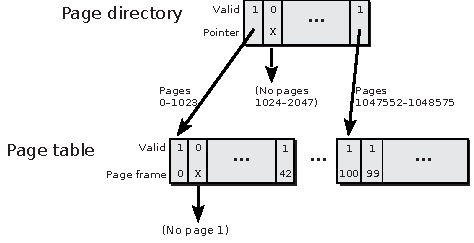
\includegraphics{hail_f0613}}
\iffalse
\centerline{\begin{graph}(311,160)(-30,0)
\graphlinecolour{0}
\grapharrowlength{5}
\fillednodesfalse
\graphnodesize{20}
\rectnode{pd0}[10,20](100,150)
\rectnode{pd1}[10,20](110,150)
\rectnode{pde}[30,20](130,150)
\rectnode{pd1023}[10,20](150,150)
\autonodetext{pd0}[w]{page directory}
\autonodetext{pde}{$\cdots$}
\rectnode{pt0.0}[10,20](50,80)
\rectnode{pt0.1}[10,20](60,80)
\rectnode{pt0.e}[30,20](80,80)
\rectnode{pt0.1023}[10,20](100,80)
\autonodetext{pt0.0}[w]{page table}
\autonodetext{pt0.e}{$\cdots$}
\diredge{pd0}{pt0.e}
\textnode{x1}(110, 122){X}[\graphlinewidth{0}\graphlinecolour{1}]
\textnode{x1n}(130, 105){\begin{tabular}{l}(no pages\\1024--2047)\end{tabular}}[\graphlinewidth{0}\graphlinecolour{1}]
\diredge{pd1}{x1}
\rectnode{pt1023.0}[10,20](150,80)
\rectnode{pt1023.1}[10,20](160,80)
\rectnode{pt1023.e}[40,20](185,80)
\autonodetext{pt1023.e}{$\cdots$}
\diredge{pd1023}{pt1023.e}
\freetext(125,80){$\cdots$}
\rectnode{p0.0}[60,20](0,10)
\autonodetext{p0.0}{page 0}
\diredge{pt0.0}{p0.0}
\textnode{x0.1}(60, 42){\begin{tabular}{c}X\\(no page 1)\end{tabular}}[\graphlinewidth{0}\graphlinecolour{1}]
\diredge{pt0.1}{x0.1}
\rectnode{p0.1023}[60,20](80,10)
\autonodetext{p0.1023}{page 1023}
\diredge{pt0.1023}{p0.1023}
\freetext(40,10){$\cdots$}
\rectnode{p1023.0}[60,20](170,10)
\autonodetext{p1023.0}{pg.~1047552}
\diredge{pt1023.0}{p1023.0}
\freetext(125,10){$\cdots$}
\rectnode{p1023.1}[60,20](235,10)
\autonodetext{p1023.1}{pg.~1047553}
\diredge{pt1023.1}{p1023.1}
\freetext(275,10){$\cdots$}
\end{graph}}
\fi
\caption{The IA-32 two-level page table has a page directory that can
  point to 1024 chunks of the page table, each of which can point to 1024 page
  frames.  The leftmost pointer leading from the leftmost chunk of the
  page table
  points to the page frame holding page~0.  Each entry can also be
  marked invalid, indicated by an X in this diagram. For example, the
  second entry in the first chunk of the page table is invalid, showing that no
  page frame holds page~1.  The same principle applies at the page
  directory level; in this example, no page frames hold pages 1024--2047, so the second page directory entry is marked invalid.}
\label{IA-32-page-table}
\end{figure}

The operating system on an IA-32 machine stores the physical base
address of the page directory in a special register, where the
hardware's page table walker can find it.  Suppose that at some later
point, the processor generates a 32-bit virtual address and presents
it to the MMU for translation.  
Figure~\ref{scan-6-8} shows the core of the translation process,
omitting the TLB and the validity checks.
\begin{figure}
\centerline{\includegraphics{hail_f0614}}
%\centerline{\def\epsfsize#1#2{0.6#1}\epsfbox{scan-6-8.eps}}
\caption{This diagram shows only the core of IA-32 paged address
  mapping, omitting the TLB and validity checks.  The virtual address
  is divided into a 20-bit page number and 12-bit offset within the
  page; the latter 12 bits are left unchanged by the translation
  process.  The page number is subdivided into a 10-bit page directory
  index and a 10-bit page table index.  Each index is multiplied by
  4, the number of bytes in each entry, and then added to the base
  physical address of the corresponding data structure, producing a
  physical memory address from which the entry is loaded.  The base
  address of the page directory comes from a register, whereas the
  base address of the page table comes from the page directory entry.}
\label{scan-6-8}
\end{figure}
In more detail, the MMU follows the following
translation process:
\begin{enumerate}
\item
Initially divide the 32-bit virtual address into its left-hand 20 bits
(the page number) and right-hand 12 bits (the offset within the page).
\item
Look up the 20-bit page number in the TLB.  If a TLB hit occurs,
concatenate the resulting page frame number with the 12-bit offset to
form the physical address.  The process is over.
\item
On the other hand, if a TLB miss occurred, subdivide the 20-bit page
number into its left-hand 10 bits (the page directory index) and its
right-hand 10 bits (the page table index).
\item
Load the page directory entry from memory; its address is four times
the page directory index plus the page directory base address, which
is taken from the special register.
\item
Check the page directory entry's valid bit.  If it is 0, then there
is no page frame holding the page in question---or any of its 1023
neighbors, for that matter.  Interrupt the processor with a page fault.
\item
Conversely, if the valid bit is 1, the page directory entry
also contains a physical base address for a chunk of page table.
\item
Load the page table entry from memory; its address is four times the
page table index plus the page table base address, which comes from the previous
step.
\item
Check the page table entry's valid bit.  If it is 0, then there is no
page frame holding the page in question.  Interrupt the processor with
a page fault.
\item
On the other hand, if the valid bit is 1, the page table entry also
contains the physical page frame number.  Load the TLB and complete
the memory access.
\end{enumerate}

This description, although somewhat simplified, shows the key
feature of the IA-32 design: it has a compact page directory, with
each entry covering a span of 4~MB.  For the 4-MB regions that are
entirely invalid, nothing further is stored.  For the regions
containing valid pages, the page directory entry points to another
compact structure containing the individual page table entries.

The
actual IA-32 design derives some additional advantages from having the page
directory entries with their 4-MB spans:
\begin{itemize}
\item
Each page directory entry can optionally point directly to a single
large 4-MB page frame, rather than pointing to a chunk of page table
entries leading indirectly to 4-KB page frames, as I described.  This
option is controlled by a page-size bit in the page directory entry.
By using this feature, the operating system can more efficiently
provide the mapping information for large, contiguously allocated
structures.
\item
Each page directory entry contains permission bits, just like the page
table entries do.  Using this feature, the operating system can mark
an entire 4-MB region of virtual address space as being read-only
more quickly, because it doesn't need to set the read-only bits
for each 4-KB page in the region.  The translation process
outlined earlier is extended to check the permission bits at each
level and signal a page fault interrupt if there is a permission
violation at either level.
\end{itemize}

The same principle used for two-level page tables can be expanded to
any greater number of levels.  If you have taken a course on data
structures, you may have seen this structure called a \vocab{trie} (or
perhaps a \foldvocab{digital}{tree} or \foldvocab{radix}{tree}).  The
virtual page number is divided into groups of consecutive bits.  Each
group of bits forms an index for use at one level of the tree,
starting with the leftmost group at the top level.  The indexing at
each level allows the chunk at the next level down to be located.

For example, the AMD64 architecture (used in the Opteron and Athlon~64
processors and later imitated by Intel under the name IA-32e) employs
four-level page tables of this kind.  Although the AMD64 is nominally
a 64-bit architecture, the virtual addresses are actually limited to
only 48 bits in the current version of the architecture.  Because the
basic page size is still 4~KB, the rightmost 12 bits are still the
offset within a page.  Thus, 36 bits remain for the virtual page
number.  Each page table entry (or similar entry at the higher levels)
is increased in size to 8 bytes, because the physical addresses
are larger than in IA-32.  Thus, a 4-KB chunk of page table can reference
only 512 pages spanning 2~MB.  Similarly, the branching factor
at each higher level of the tree is 512.  Because 9 bits are needed
to select from 512 entries, it follows that the 36-bit virtual page
number is divided into four groups of 9 bits each, one for each
level of the tree.

Achieving adequate performance with a four-level page table is
challenging. The AMD designers will find this challenge intensified if
they extend their architecture to full 64-bit virtual addresses, which
would require two more levels be added to the page table.  Other
designers of 64-bit processors have made different choices: Intel's
Itanium uses either linear page tables or hashed page tables, and the
PowerPC uses hashed page tables.

\subsection{Hashed Page Tables}\label{hashed-page-tables-section}

You have seen that linear page tables and multilevel page tables have
a strong family resemblance.  Both designs rely on the assumption that valid
and invalid pages occur in large clumps.  As a result, each allows you to
finesse the dilemma of wanting to store page table entries for
successive pages consecutively in memory, yet not wanting to waste
storage on invalid entries.  You store page table entries
consecutively within each chunk of the table and omit storage for
entire chunks of the table.

Suppose you take a radical approach and reject the starting
assumption.  You will still assume that the address space is sparsely occupied;
that is, many page table entries are invalid and should not be stored.
(After all, no one buys $2^{64}$ bytes of RAM for their 64-bit
processor.)  However, you will no longer make any assumption about
clustering of the valid and invalid pages---they might be scattered
randomly throughout the whole address space.  This allows greater flexibility for the designers of
runtime environments.  As a consequence, you will have
to store individual valid page table entries, independent of their
neighbors.

Storing only individual valid page table entries without storing any
of the invalid entries takes away the primary tool used by the
previous approaches for locating
entries.  You can no longer find page $n$'s entry by indexing $n$
elements into an array---not even within each chunk of the address
space.  Therefore, you need to use an entirely different approach to
locating page table entries.  You can store them in a hash table, known
as a \foldvocab{hashed}{page table}.

A hashed page table is an array of \foldvocabs{hash}{bucket}, each of
which is a fixed-sized structure that can hold some small number of
page table entries.  (In the Itanium architecture, each bucket holds
one entry, whereas in the PowerPC, each bucket holds eight entries.)
Unlike the linear page table, this array of buckets does not have a
private location for each virtual page number; as such, it can be much
smaller, particularly on 64-bit architectures.

Because of this reduced array size, the page number cannot be directly
used as an index into the array.  Instead, the page number is first fed through a
many-to-one function, the \vocab{hash function}.  That is, each page
gets assigned a specific hash bucket by the hash function, but many
different pages get assigned the same bucket.  The simplest plausible
hash function would be to take the page number modulo the number of
buckets in the array.  For example, if there are 1000000 hash buckets,
then the page table entries for pages 0, 1000000, 2000000, and so
forth would all be assigned to bucket~0, while pages 1, 1000001,
2000001, and so forth would all be assigned to bucket~1.

The performance of the table relies on the assumption that only a few
of the pages assigned to a bucket will be valid and hence have page
table entries stored.  That is, the assumption is that only rarely
will multiple valid entries be assigned to the same bucket, a
situation known as a \foldvocab{hash}{collision}.  To keep collisions
rare, the page table size needs to scale with the number of valid page
table entries.  Luckily, systems with lots of valid page table entries
normally have lots of physical memory and therefore have room for a
bigger page table.

Even if collisions are rare, there must be some mechanism
for handling them.  One immediate consequence is that each page table
entry will now need to include an indication of which virtual page
number it describes.  In the linear and multilevel page tables, the
page number was implicit in the location of the page table entry.
Now, any one of many different page table entries could be assigned to
the same location, so each entry needs to include an identifying tag, much like
in the TLB.

For an unrealistically small example of using a hashed page table, we can return to
Figure~\ref{example-mapping} on page~\pageref{example-mapping}.
Suppose you have a hashed page table with four buckets, each capable of
holding one entry.  Each of the four entries will contain both a
virtual page number and a corresponding physical page frame number.  If the
hash function consists of taking the page number modulo 4, the table
would contain approximately the information shown in Figure~\ref{example-hash-page-table}.
\begin{figure}
\centerline{\begin{tabular}{|c|c|c|}
\hline\textbf{Valid}&\textbf{Page}&\textbf{Page Frame}\\\hline
1&0&1\\\hline
1&1&0\\\hline
1&6&3\\\hline
0&X&X\\\hline
\end{tabular}}
\caption{Each entry in a hashed page table is in a location determined
by feeding the page number through a hash function.  In this example,
the hash function consists of taking the page number modulo the number
of entries in the table, 4.  Consider the entry recording
that page~6 is held by page frame~3.  This entry is in position~2
within the table (counting from 0) because the remainder when 6 is divided by 4 is 2.}
\label{example-hash-page-table}
\end{figure}

The possibility of collisions has another consequence, beyond
necessitating page number tags.  Even if collisions occur, each valid
page table entry needs to be stored somewhere.  Because the colliding
entries cannot be stored in the same location, some alternative
location needs to be available.  One possibility is to have
alternative locations within each hash bucket; this is why the PowerPC
has room for eight page table entries in each bucket.  Provided no
collision involves more than this number of entries, they can all be
stored in the same bucket.  The PowerPC searches all entries in the
bucket, looking for one with a matching tag.

If a collision involving more than eight entries occurs on a
PowerPC, or any collision at all occurs on an Itanium processor, the
collision cannot be resolved within the hash bucket.
To handle such collisions, the operating system can allocate some extra memory and
chain it onto the bucket in a linked list.  This will be an
expensive but rare occurrence.  As a result, hardware page table
walkers do not normally handle this case.  If the walker does not find
a matching tag within the bucket, it uses an interrupt to transfer
control to the operating system, which is in charge of searching
through the linked list.

You have now seen two reasons why the page table entries in hashed
page tables need to be larger than those in linear or multilevel page
tables.  The hashed page table entries need to contain virtual page
number tags, and each bucket needs a pointer to an
overflow chain. As a
result of these two factors and the addition of some extra features,
the Itanium architecture uses 32-byte entries for hashed page tables
versus 8-byte entries for linear page tables.

Incidentally, the fact that the Itanium architecture supports two
different page table formats suggests just how hard it is to select
one.  Research continues into the relative merits of the different
formats under varying system workloads.  As a result of this research,
future systems may use other page table formats beyond those described
here, though they are likely to be variants on one of these themes.
Architectures such as MIPS that have no hardware page table walker are
excellent vehicles for such research, because they allow the operating
system to use any page table format whatsoever.

Some operating systems treat a hashed page table as a
\foldvocab{software}{TLB}, a table similar to the hardware's TLB in
that it holds only selected page table entries.  In this case, no
provision needs to be made for overfull hash buckets; the entries
that don't fit can simply be omitted.  A slower multilevel page table
provides a comprehensive fallback for misses in the software TLB.
This alternative is particularly
attractive when porting an operating system (such as Linux) that was
originally developed on a machine with multilevel page tables.

\subsection{Segmentation}\label{vm-segmentation-section}

Thus far, I have acted as though virtual memory were synonymous with
paging.  Today, that is true.  However, when virtual memory was first
developed in the 1960s, there were two competing approaches: paging
and \vocab{segmentation}.  Some systems (notably Multics) also included a
hybrid of the two.  Thus, seen historically, segmentation was both a
competitor and a collaborator of paging.  Today, segmentation remains
only in vestigial form.  The IA-32 architecture still contains full
support for segmentation, but no common operating system uses it, and
the successor architectures (Itanium and AMD64) have dropped it.  As
such, this subsection can be omitted with no great loss.

Recall that the basic premise of virtual memory is that a process uses
addresses as names for objects, whereas memory uses addresses as
routing information for storage locations.  The defining property of
segmentation is that the processor's virtual addresses name
objects using two granularities: each virtual address names both
an aggregate object, such as a table or file, and a particular
location within that object, such as a table entry or a byte within a
file.  This is somewhat analogous to my name, ``Max Hailperin,''
which identifies both the family to which I belong (Hailperin), and
the particular person within that family (Max).

The aggregate objects, such as tables or files, that have names akin
to family names are called \vocabs{segment}.  Each process refers to
its segments by segment number.  Each virtual address is divided into
two parts: some number of bits are a segment number, and the remaining
bits are a location within that segment.

On the surface, segmented virtual addresses may not seem very
different from paged ones.  After all, you saw that paged virtual
addresses are also divided into two parts: a page number and an offset
within that page.  For example, a 32-bit address might be divided into a
20-bit page number and a 12-bit offset within the page.  The key
difference is that pages are purely an implementation detail; they do
not correspond to logical objects such as files, stacks, or tables.

Because segments correspond to logical objects, they cannot have a
fixed size, such as 4~KB.  Each segment will have its own natural
size.  For example, each file a process accesses might be mapped into
the virtual address space as its own segment.  If so, the segment
sizes will need to match the file sizes, which could be quite
arbitrary.

A system employing pure segmentation maps each segment into a
contiguous range of physical memory.  Instead of a page table, the
system uses a segment table, which specifies for each segment number
the starting physical address, the size, and the permissions.

Unlike paging, pure segmentation does not provide for flexible
allocation of physical memory; external fragmentation may occur, where
it is hard to find enough contiguous free memory to accommodate a
segment.  In addition, pure segmentation does not provide good support for
moving inactive information to disk, because only an entire segment
can be transferred to or from disk.

Because of these and similar problems, segmentation can be combined
with paging.  Each process uses two-part addresses containing segment
numbers and offsets.  The MMU translates each of these addresses in
two stages using both a segment table and a page table.  The end
result is an offset within a physical memory page frame. Thus, each
segment may occupy any available page frames, even if they are not
contiguous, and individual pages of the segment may be moved to disk.

Systems have combined segmentation with paging in two slightly
different ways, one exemplified by the IA-32 architecture and the
other by the Multics system.  The key difference is whether all the
segments share a single page table, as in the IA-32, or are given
individual page tables, as in Multics.

Figure~\ref{scan-6-9} shows how segmentation and paging are used
together in the IA-32 architecture's MMU.
\begin{figure}
\centerline{\includegraphics{hail_f0616}}
%\centerline{\def\epsfsize#1#2{0.6#1}\epsfbox{scan-6-9.eps}}
\caption{The IA-32 architecture combines segmentation and paging
  using a single page table for all the segments.  The segment table
  is used to translate the segment number into a base address, to
  which the offset within the segment is added, yielding a linear
  address.  The linear address is then translated to a physical
  address using the unified page table, as shown in greater detail in Figure~\ref{scan-6-8}.}
\label{scan-6-9}
\end{figure}
When the IA-32 MMU translates a virtual address, it starts by looking up
the segment number in a segment table, yielding a starting address
for the segment, a length, and permissions, just like in systems that
use pure segmentation.  Assuming the permissions are OK and the offset
is legal with regard to the length, the MMU adds the segment's
starting address to the offset.  However, rather than treating the sum
as a physical address, the MMU treats it as a paged virtual address,
of the sort I have described in previous subsections.  In IA-32
terminology, this address is known as a \foldvocab{linear}{address}.  The
MMU looks up the linear address in a single page table, shared by all
the segments, in order to locate the appropriate page frame.

Figure~\ref{scan-6-10} shows an alternative method of combining
segmentation and paging, which was used in the \index{Multics}Multics system.
\begin{figure}
\centerline{\includegraphics{hail_f0617}}
%\centerline{\def\epsfsize#1#2{0.6#1}\epsfbox{scan-6-10.eps}}
\caption{The Multics system combines segmentation and paging using a
  separate page table for each segment.  The segment table is used to
  find the appropriate page table, which is then used to translate the
  address within the segment.}
\label{scan-6-10}
\end{figure}
The Multics approach also starts by looking up the segment number in a
segment table, which again provides information on the segment's
length and permissions to allow the MMU to check the access for
legality.  However, this segment table does not contain a starting
address for the segment; instead, it contains a pointer to the
segment's private page table.  The MMU uses this segment-specific page
table to translate the offset within the segment, using techniques of
the sort you saw in previous subsections.  The end result is again an
offset within a page frame.

Which approach is simpler for the operating system to manage?  On the
surface, the IA-32 approach looks simpler, because it uses only a
single page table instead of one per segment.  However, it has a
significant disadvantage relative to the Multics approach.  Remember
that both approaches allow space in physical memory to be flexibly
allocated in individual, non-contiguous page frames.  However, the
IA-32 approach forces each segment to be allocated a single contiguous
region of address space at the level of linear addresses.  Thus, the
IA-32 approach forces the operating system to deal with the
complexities of contiguous allocation, with its potential for external
fragmentation.

Unlike pure segmentation, which is undeniably inferior to paging, the
combination of segmentation and paging seems attractive, as it combines
segmentation's meaningful units for protection and sharing with
paging's smaller fixed-size units for space allocation and data transfer.
However, many of the same protection and sharing features can be
simulated using paging alone.  Probably as a result of this, many
hardware designers decided the cost of segmentation, in both money and
performance, was not justified by the gain.  Therefore, they provided support
only for paging.  This created a disincentive for the use of
segmentation in operating systems; all popular operating systems (such as UNIX,
Microsoft Windows, and Linux) are designed to be portable across
multiple hardware architectures, some of which don't support
segmentation.  As a result, none of these operating systems makes
any use of segmentation, even on systems where it is supported.  This
completes a cycle of disincentives; designers of modern architectures
have no reason to support segmentation, because modern operating
systems do not use it.

Although modern architectures no longer support segmentation, they do have one
feature that is reminiscent of the combination of segmentation and
paging.  Recall that TLBs and hashed page tables use ASIDs to tag page
translations so that translations from different processes can
coexist.  I said that a special register holds the ASID of the
current process.  In actuality, many modern architectures allow each
process to use several different ASIDs; the top few bits of each
virtual address select one of a group of ASID registers.  Thus,
address translation occurs in two steps.  First, the top bits of the
address are translated to an ASID; then the ASID and the remaining
bits are translated into a page frame and offset.  If the operating
system sets up several processes to use the same ASID for a shared
library, they will wind up sharing not only the page frames, but also
the page table and TLB entries.  This is akin to processes sharing a
segment.  However, unlike segmentation, it is invisible at the
application level.  Also, the number of segments (ASIDs) per process
may be quite limited: eight on the Itanium and 16 on the 32-bit
version of PowerPC.

\section{Policies for Virtual Memory}\label{vm-policies-section}

Thus far, I have defined virtual memory, explained its usefulness,
and shown some of the mechanisms typically used to map pages to page
frames.  Mechanisms alone, however, are not enough.  The operating
system also needs a set of policies describing how the mechanisms are
used.  Those policies provide answers for the following questions:
\begin{itemize}
\item
At what point is a page assigned a page frame?  Not until the page is
first accessed, or at some earlier point?  This decision is
particularly performance critical if the page needs to be fetched from
disk at the time it is assigned a page frame.  For this reason, the
policy that controls the timing of page frame assignment is normally
called the \vocab{fetch policy}.
\item
Which page frame is assigned to each page?  I have said that each
page may be assigned any available frame, but some assignments may
result in improved performance of the processor's cache memory.  The
policy that selects a page frame for a page is known as the
\vocab{placement policy}.
\item
If the operating system needs to move some inactive page to disk in
order to free up a page frame, which page does it choose?  This is
known as the the \vocab{replacement policy}, because the page being
moved to disk will presumably be replaced by a new page---that being
the motivation for freeing a page frame.
\end{itemize}

All of these policies affect system performance in ways that are quite
workload dependent.  For example, a replacement policy that performs well
for one workload might perform terribly on another; for instance, it might consistently choose to
evict a page that is accessed again a moment later.  As such, these
policies need to be chosen and refined through extensive
experimentation with many real workloads.  In the following
subsections, I will focus on a few sample policies that are
reasonably simple and have performed adequately in practice.

\subsection{Fetch Policy}
\label{fetch-policy}

The\index{fetch policy} operating system has wide latitude regarding when each page is
assigned a page frame.  At one extreme, as soon as the operating
system knows about a page's existence, it could assign a page frame.
For example, when a process first starts running, the operating system
could immediately assign page frames for all the pages holding the
program and its statically allocated data.  Similarly, when a process
asks the operating system to map a file into the virtual memory
address space, the operating system could assign page frames for the
entire file.  At the other extreme, the operating system could wait
for a page fault caused by an access to a page before assigning that
page a page frame.  In between these extremes lies a range of realistic
fetch policies that try to stay just a little ahead of the process's
needs.

Creating all page mappings right away would conflict with many of the
original goals for virtual memory, such as fast start up of programs
that contain large but rarely used portions.  Therefore,
one extreme policy can be discarded.  The other, however, is a reasonable
choice under some circumstances.  A system is said to use
\foldvocab{demand}{paging} if it creates the mapping for each page in
response to a page fault when accessing that page.  Conversely, it
uses \vocab{prepaging} if it attempts to anticipate future page use.

Demand paging has the advantage that it will never waste time creating
a page mapping that goes unused; it has the disadvantage that it
incurs the full cost of a page fault for each page.  On balance, demand paging is
particularly appropriate under the following circumstances:
\begin{itemize}
\item
If the process exhibits limited spatial locality, the operating system
is unlikely to be able to predict what pages are going to be used
soon.  This makes paging in advance of demand less likely to pay off.
\item
If the cost of a page fault is particularly low, even moderately
accurate predictions of future page uses may not pay off, because so
little is gained each time a correct prediction allows a page fault to
be avoided.
\end{itemize}

The Linux operating system uses demand paging in exactly the
circumstances suggested by this analysis.  The fetch policy makes a
distinction between zero-filled pages and those that are read from a
file, because the page fault costs are so different.  Linux uses
demand paging for zero-filled pages because of their comparatively
low cost.  In contrast, Linux ordinarily uses a variant of prepaging
(which I explain in the remainder of this subsection) for files mapped into virtual memory.  This
makes sense because reading from disk is slow.  However, if the
application programmer notifies the operating system that a particular
memory-mapped file is going to be accessed in a ``random'' fashion,
then Linux uses demand paging for that file's pages.  The programmer
can provide this information using the
\index{madvise@\verb"|madvise"|}\verb|madvise| procedure.

The most common form of prepaging is \foldvocab{clustered}{paging}, in
which each page fault causes a cluster of neighboring pages to be
fetched, including the one incurring the fault.  Clustered paging is
also called \vocab{read around}, because pages around the faulting
page are read.  (By contrast, \vocab{read ahead} reads the faulting
page and later pages, but no earlier ones.)

The details of clustered paging vary between operating systems.  Linux
reads a cluster of sixteen pages aligned to start with a multiple of 16.
For example, a page fault on any of the first sixteen pages of a file will
cause those sixteen pages to be read.  Thus, the extra fifteen pages can be all
before the faulting page, all after it, or any mix.  Microsoft Windows
uses a smaller cluster size, which depends in part on the kind of page
incurring the fault: instructions or data.  Because instruction
accesses generally exhibit more spatial locality than data accesses,
Windows uses a larger cluster size for instruction pages than for data
pages.

Linux's read around is actually a slight variant on the prepaging
theme.  When a page fault occurs, the fault handler fetches a whole
cluster of pages into RAM but only updates the faulting page table
entry.  The other pages are in RAM but not mapped into any virtual
address space; this status is known as the \vocab{page cache}.
Subsequent page faults can quickly find pages in the page cache.  Thus, read around
doesn't decrease the total number of page faults, but converts many
from \foldvocabs{major}{page fault} (reading disk) to
\foldvocabs{minor}{page fault} (simply updating the page table).

Because reading from disk takes about 10 milliseconds and
because reading sixteen pages takes only slightly longer than reading one,
the success rate of prepaging doesn't need to be especially high for
it to pay off.  For example, if the additional time needed to read and
otherwise process each prepaged page is half a millisecond, then
reading a cluster of sixteen pages, rather than a single page, adds 7.5
milliseconds.  This would be more than repaid if even a single one of
the fifteen additional pages gets used, because the prepaging would avoid a 10-millisecond disk
access time.

\subsection{Placement Policy}

Just\index{placement policy} as the operating system needs to determine when to make a
page resident (on demand or in advance), it needs to decide
where the page should reside by selecting one of the unused page
frames. This choice influences the physical memory addresses that will
be referenced and can thereby influence the miss rate of the \index{cache
memory}cache memory hardware.

Although cache performance is the main issue in desktop systems, there
are at least two other reasons why the placement policy may matter.
In \index{ccNUMA}\index{NUMA}large-scale multiprocessor systems, main memory is distributed
among the processing nodes.  As such, any given processor will have
some page frames it can more rapidly access.  Microsoft's Windows
Server 2003 takes this effect into account when allocating page
frames.  Another issue, likely to become more important in the future,
is the potential for \index{power}\index{energy}energy savings if all accesses can be confined to
only a portion of memory, allowing the rest to be put into standby
mode.

To explain why the placement policy influences cache miss rate, I
need to review cache memory organization.  An idealized cache would
hold the $n$ most recently accessed blocks of memory, where $n$ is the
cache's size.  However, this would require each cache access to
examine all $n$ blocks, looking to see if any of them contains the
location being accessed.  This approach, known as \foldvocab{full}{associativity},
is not feasible for realistically large caches.  Therefore, real
caches restrict any given memory location to only a small set of
positions within the cache; that way, only those positions need to be
searched.  This sort of cache is known as \vocabindex{set-associative}{set associativity}\index{associativity, set}.  For
example, a two-way set-associative cache has two alternative locations where
any given memory block can be stored.  Many caches, particularly
those beyond the first level (L1), use the physical address rather than
the virtual address to select a set.

Consider what would happen if a process repeatedly accesses three
blocks of memory that have the misfortune of all competing for the
same set of a two-way set-associative cache.  Even though the cache may
be large---capable of holding far more than the three blocks that are
in active use---the miss rate will be very high.  The standard description for
this situation is to say the cache is
suffering from \foldvocabes{conflict}{miss} rather than \foldvocabes{capacity}{miss}.  Because
each miss necessitates an access to the slower main memory, the high
rate of conflict misses will significantly reduce performance.

The lower the cache's associativity, the more likely conflict misses
are to be a problem.  Thus, careful page placement was more important
in the days when caches were external to the main microprocessor chips,
as external caches are often of low associativity.  Improved
semiconductor technology has now allowed large caches to be integrated
into microprocessors, making higher associativity economical and
rendering placement policy less important.

Suppose, though, that an operating system does wish to allocate page
frames to reduce cache conflicts.  How should it know which
pages are important to keep from conflicting?  One common approach is
to assume that pages that would not conflict without virtual memory
address translation should not conflict even with address translation;
this is known as \foldvocab{page}{coloring}.  Another common approach
is to assume that pages that are mapped into page frames soon after
one another are likely to also be accessed in temporal proximity;
therefore, they should be given nonconflicting frames.  This is known
as \vocab{bin hopping}.

The main argument in favor of page coloring is that it leaves intact
any careful allocation done at the level of virtual addresses.  Some
compiler authors and application programmers are aware of the
importance of avoiding cache conflicts, particularly in
high-performance scientific applications, such as weather forecasting.
For example, the compiler or programmer may pad each row of an array
with a little wasted space so that iterating down a column of the
array won't repeatedly access the same set of the cache.  This kind of
cache-conscious data allocation will be preserved by page coloring.

The main argument in favor of bin hopping is that experimental evidence
suggests it performs better
than page coloring does, absent cache-conscious data allocation.  This may be because page coloring is less
flexible than bin hopping, providing only a way of deciding on the
most preferred locations in the cache for any given page, as opposed
to ranking all possible locations from most preferred to least.

\subsection{Replacement Policy}

Conceptually, a replacement policy chooses a page to evict every time
a page is fetched with all page frames in use.  However, operating
systems typically try do some eviction in advance of actual demand,
keeping an inventory of free page frames.  When the inventory
drops below a \vocab{low-water mark}, the replacement policy starts
freeing up page frames, continuing until the inventory surpasses a
\vocab{high-water mark}.  Freeing page frames in advance of demand has
three advantages:
\begin{itemize}
\item
Last-minute freeing in response to a page fault will further delay the
process that incurred the page fault.  In contrast, the operating
system may schedule proactive work to maintain an inventory of free
pages when the hardware is otherwise idle, improving response time and
throughput.
\item
Evicting dirty pages requires writing them out to disk first.  If the
operating system does this proactively, it may be able to write back
several pages in a single disk operation, making more efficient use of
the disk hardware.
\item
In the time between being freed and being reused, a page frame can
retain a copy of the page it most recently held.  This allows the
operating system to inexpensively recover from poor replacement
decisions by retrieving the page with only a minor page fault instead
of a major one.  That is, the page can be retrieved by mapping it
back in without reading it from
disk.  You will see that this is particularly important if the MMU does
not inform the replacement policy which pages have been recently
referenced.
\end{itemize}

In a real operating system, a page frame may go through several
temporary states between when it is chosen for replacement and when it
is reused.  For example, Microsoft Windows may move a replaced page
frame through the following four inventories of page frames, as
illustrated in Figure~\ref{scan-6-11}:
\begin{figure}
\centerline{\includegraphics{hail_f0618}}
%\centerline{\def\epsfsize#1#2{0.6#1}\epsfbox{scan-6-11.eps}}
\caption{Each page frame in Microsoft Windows that is not referenced from
  a page table is included in one of the four page lists.  Page frames
  circulate as shown here.  For example, the system can use a soft
  page fault to recover a page frame from the modified or standby page
  list, if the page contained in that page frame proves to still be
  needed after having been evicted by the replacement policy.}
\label{scan-6-11}
\end{figure}
\begin{itemize}
\item
When the replacement policy first chooses a dirty page frame, the
operating system moves
the frame from a process's page table to the \vocab{modified page list}.  The
modified page list retains information on the previous page mapping
so that a minor page fault can retrieve the page.  (Microsoft calls this a
\foldvocab{soft}{page fault}.)
\item
If a page frame remains in the
modified page list long enough, a system thread known as the \vocab{modified
page writer} will write the contents out to disk and move the frame to
the \vocab{standby page list}.  A page frame can also move directly from a
process's page table to the standby page list if the replacement
policy chooses to evict a clean page.  The standby page list again
retains the previous mapping information so that a soft page fault
can inexpensively recover a prematurely evicted page.
\item
If a page frame remains on standby for long enough without being
faulted back into use, the operating system moves it to the \vocab{free page
list}. This list provides page frames for the system's \vocab{zero page thread}
to proactively fill with zeros, so that zero-filled pages will be
available to quickly respond to page faults, as discussed earlier.
The operating system also prefers to use a page frame from the free
list when reading a page in from disk.
\item
Once the zero page thread has filled a free page frame with zeros, it
moves the page frame to the \vocab{zero page list}, where it will remain until
mapped back into a process's page table in response to a page fault.
\end{itemize}

Using a mechanism such as this example from Windows, an operating system keeps an
inventory of page frames and thus need not evict a page every time it
fetches a page.  In order to keep the size of this inventory
relatively stable over the long term, the operating system balances
the rate of page replacements with the rate of page fetches.  It can
do this in either of two different ways, which lead to the two major
categories of replacement policies, \vocab{local replacement} and
\vocab{global replacement}.

Local replacement keeps the rate of page evictions and page fetches
balanced individually for each process.  If a process incurs many page
faults, it will have to relinquish many of its own page frames, rather
than pushing other processes' pages out of their frames.  The
replacement policy chooses which page frames to free only from those
held by a particular process.  A separate allocation policy decides how
many page frames each process is allowed.

Global replacement keeps the rate of page evictions and page fetches
balanced only on a system-wide basis.  If a process incurs many page
faults, other process's pages may be evicted from their frames.  The
replacement policy chooses which page frames to free from all the page
frames, regardless which processes they are used by.  No separate page
frame allocation policy is needed, because the replacement policy and
fetch policy will naturally wind up reallocating page frames between
processes.

Of the operating systems popular today, Microsoft Windows uses local
replacement, whereas all the members of the UNIX family, including
Linux and Mac OS~X, use global replacement.  Microsoft's choice of a
local replacement policy for Windows was part of a broader pattern of
following the lead of Digital Equipment Corporation's VMS operating
system, which has since become HP's OpenVMS.  The key reason why VMS's
designers chose local replacement was to prevent poor locality of
reference in one process from greatly hurting the performance of other
processes.  Arguably, this performance isolation is less relevant for
a typical Windows desktop or server workload than for VMS's multi-user
real-time and timesharing workloads.  Global replacement is simpler,
and it more flexibly adapts to processes whose memory needs
are not known in advance.  For these reasons, it tends to be more
efficient.

Both local and global replacement policies may be confronted with a
situation where the total size of the
processes' working sets exceeds the
number of page frames available.  In the case of local replacement,
this manifests itself when the allocation policy cannot allocate a
reasonable number of page frames to each process.  In the case
of global replacement, an excessive demand for memory is manifested as
\vocab{thrashing}, that is, by the system spending essentially all its time
in paging and process switching, producing extremely low throughput.

The traditional solution to excess memory demand is \vocab{swapping}.
The operating system picks some processes to evict entirely from
memory, writing all their data to disk.  Moreover, it removes those
processes' threads from the scheduler's set of runnable threads, so
that they will not compete for memory space.  After running the
remaining processes for a while, the operating system swaps some of
them out and some of the earlier victims back in.  Swapping adds to
system complexity and makes scheduling much choppier; therefore,
some global replacement systems such as Linux omit it and rely on
users to steer clear of thrashing.  Local replacement systems such as
Microsoft Windows, on the other hand, have little choice but to
include swapping.  For simplicity, I will not discuss swapping
further in this text.  You should know what it is, however, and should
also understand that some people incorrectly call paging swapping; for
example, you may hear of Linux swapping, when it really is paging.
That is, Linux is moving individual pages of a process's address space
to disk and back, rather than moving the entire address space.

Having seen some of the broader context into which replacement
policies fit, it is time to consider some specific policies.
I will start with one that is unrealistic but which provides a
standard against which other, more realistic policies can be measured.
If the operating system knew in advance the full sequence of virtual
memory accesses, it could select for replacement the page that has its
next use furthest in the future.  This turns out to be more than just
intuitively appealing: one can mathematically prove that it optimizes
the number of demand fetches.  Therefore, this replacement policy is
known as \vocab{optimal replacement} (\vocab{OPT}).

Real operating systems don't know future page accesses in advance.
However, they may have some data that allows the probability of
different page accesses to be estimated.  Thus, a replacement policy
could choose to evict the page estimated to have the longest time
until it is next used.  As one special case of this, consider a
program that distributes its memory accesses across the pages
randomly but with unequal probabilities, so that some pages are more
frequently accessed than others.  Suppose that these probabilities
shift only slowly. In that case, pages which have been accessed
frequently in the recent past are likely to be accessed again soon,
and conversely, those that have not been accessed in a long while are
unlikely to be accessed soon.  As such, it makes sense to replace the
page that has gone the longest without being accessed.  This
replacement policy is known as \vocab{Least Recently Used} (\vocab{LRU}).

LRU replacement is more realistic than OPT, because it uses only
information about the past, rather than about the future.  However,
even LRU is not entirely realistic, because it requires keeping a list
of page frames in order by most recent access time and updating that
list on every memory access.  Therefore, LRU is used much as OPT is,
as a standard against which to compare other policies.  However, LRU
is not a gold standard in the same way that OPT is; while OPT is
optimal among all policies, LRU may not even be optimal among policies
relying only on past activity.  Real processes do not access pages
randomly with slowly shifting probability distributions.  For
example, a process might repeatedly loop through a set of pages, in
which case LRU will perform terribly, replacing the page that will be
reused soonest.  Nonetheless, LRU tends to perform reasonably well
in many realistic settings; therefore, many other replacement policies try
to approximate it.  While they may not replace the least recently used
page, they will at least replace a page that hasn't been used very
recently.

Before considering realistic policies that approximate LRU, I should
introduce one other extremely simple policy, which can serve as a
foundation for an LRU-approximating policy, though it isn't one
itself. The simple policy is known as \vocab{first in,
first out replacement} (\vocab{FIFO}).  The name tells the whole story: the operating
system chooses for replacement whichever page frame has been holding
its current page the longest.  Note the difference between FIFO and
LRU; FIFO chooses the page that was fetched the longest ago, even if
it continues to be in frequent use, whereas LRU chooses the page that
has gone the longest without access.
Figure~\ref{replacement-comparison} shows an example where LRU
outperforms FIFO and is itself outperformed by OPT.
This performance ordering is not universal; in Exercises \ref{FIFO-better-exercise} and \ref{OPT-tied-exercise},
you can show that FIFO sometimes outperforms LRU and that OPT does
not always perform strictly better than the others.
\begin{figure}
\centerline{\includegraphics{hail_f0619}}
\iffalse
\centerline{\begin{graph}(344,185)
\graphlinecolour{0}
\fillednodesfalse
\graphnodesize{20}
\squarenode{ot0}(40,150)
\squarenode{ob0}(40,130)
\squarenode{lt0}(40,90)
\squarenode{lb0}(40,70)
\squarenode{ft0}(40,30)
\squarenode{fb0}(40,10)
\squarenode{ot1}(82,150)
\squarenode{ob1}(82,130)
\squarenode{lt1}(82,90)
\squarenode{lb1}(82,70)
\squarenode{ft1}(82,30)
\squarenode{fb1}(82,10)
\squarenode{ot2}(124,150)
\squarenode{ob2}(124,130)
\squarenode{lt2}(124,90)
\squarenode{lb2}(124,70)
\squarenode{ft2}(124,30)
\squarenode{fb2}(124,10)
\squarenode{ot3}(166,150)
\squarenode{ob3}(166,130)
\squarenode{lt3}(166,90)
\squarenode{lb3}(166,70)
\squarenode{ft3}(166,30)
\squarenode{fb3}(166,10)
\squarenode{ot4}(208,150)
\squarenode{ob4}(208,130)
\squarenode{lt4}(208,90)
\squarenode{lb4}(208,70)
\squarenode{ft4}(208,30)
\squarenode{fb4}(208,10)
\squarenode{ot5}(250,150)
\squarenode{ob5}(250,130)
\squarenode{lt5}(250,90)
\squarenode{lb5}(250,70)
\squarenode{ft5}(250,30)
\squarenode{fb5}(250,10)
\squarenode{ot6}(292,150)
\squarenode{ob6}(292,130)
\squarenode{lt6}(292,90)
\squarenode{lb6}(292,70)
\squarenode{ft6}(292,30)
\squarenode{fb6}(292,10)
\squarenode{ot7}(334,150)
\squarenode{ob7}(334,130)
\squarenode{lt7}(334,90)
\squarenode{lb7}(334,70)
\squarenode{ft7}(334,30)
\squarenode{fb7}(334,10)
\freetext(15,140){OPT}
\freetext(15,80){LRU}
\freetext(15,20){FIFO}
\freetext(61,180){1}
\freetext(61,140){m}
\freetext(61,80){m}
\freetext(61,20){m}
\freetext(103,180){2}
\freetext(103,140){m}
\freetext(103,80){m}
\freetext(103,20){m}
\freetext(145,180){1}
\freetext(145,140){h}
\freetext(145,80){h}
\freetext(145,20){h}
\freetext(187,180){3}
\freetext(187,140){m}
\freetext(187,80){m}
\freetext(187,20){m}
\freetext(229,180){1}
\freetext(229,140){h}
\freetext(229,80){h}
\freetext(229,20){m}
\freetext(271,180){2}
\freetext(271,140){m}
\freetext(271,80){m}
\freetext(271,20){m}
\freetext(313,180){3}
\freetext(313,140){h}
\freetext(313,80){m}
\freetext(313,20){m}
\autonodetext{ot1}{1}
\autonodetext{lt1}{1}
\autonodetext{ft1}{1}
\autonodetext{ot2}{1}
\autonodetext{ob2}{2}
\autonodetext{lt2}{1}
\autonodetext{lb2}{2}
\autonodetext{ft2}{1}
\autonodetext{fb2}{2}
\autonodetext{ot3}{1}
\autonodetext{ob3}{2}
\autonodetext{lt3}{1}
\autonodetext{lb3}{2}
\autonodetext{ft3}{1}
\autonodetext{fb3}{2}
\autonodetext{ot4}{1}
\autonodetext{ob4}{3}
\autonodetext{lt4}{1}
\autonodetext{lb4}{3}
\autonodetext{ft4}{3}
\autonodetext{fb4}{2}
\autonodetext{ot5}{1}
\autonodetext{ob5}{3}
\autonodetext{lt5}{1}
\autonodetext{lb5}{3}
\autonodetext{ft5}{3}
\autonodetext{fb5}{1}
\autonodetext{ot6}{2}
\autonodetext{ob6}{3}
\autonodetext{lt6}{1}
\autonodetext{lb6}{2}
\autonodetext{ft6}{2}
\autonodetext{fb6}{1}
\autonodetext{ot7}{2}
\autonodetext{ob7}{3}
\autonodetext{lt7}{3}
\autonodetext{lb7}{2}
\autonodetext{ft7}{2}
\autonodetext{fb7}{3}
\end{graph}}
\fi
\caption{In this comparison of the OPT, LRU, and FIFO replacement
  policies, each pair of boxes represents the two page frames
  available on an unrealistically small system.  The numbers within
  the boxes indicate which page is stored in each page frame.  The
  numbers across the top are the reference sequence, and the letters h
  and m indicate hits and misses.  In this example, LRU performs
  better than FIFO, in that it has one more hit.  OPT performs even
  better, with three hits.}
\label{replacement-comparison}
\end{figure}

FIFO is not a very smart policy; in fact, early simulations showed
that it performs comparably to random replacement.  Beyond this
mediocre performance, one sign that FIFO isn't very smart is that it
suffers from \vocab{Belady's anomaly}: increasing the number of page
frames available may increase the number of page faults, rather than
decreasing it as one would expect.  In Exercise~\ref{Belady-exercise},
you can generate an example of this counterintuitive performance
phenomenon.

Both OPT and LRU are immune from Belady's anomaly, as are all other
members of the class of \vocab{stack algorithms}.  A stack algorithm is
a replacement policy with the property that if you run the same
sequence of page references on two systems using that replacement
policy, one with $n$ page frames and the other with $n+1$, then at each
point in the reference sequence the $n$ pages that occupy page frames
on the first system will also be resident in page frames on the second
system.  For example, with the LRU policy, the $n$ most recently
accessed pages will be resident in one system, and the $n+1$ most
recently accessed pages will be resident in the other. Clearly the $n+1$ most recently
accessed pages include the $n$ most recently accessed pages.  In
Exercise~\ref{OPT-stack-exercise}, you can come up with a similar
justification for my claim that OPT is a stack algorithm.

Recall that at the beginning of this subsection, I indicated that
page frames chosen for replacement are not immediately reused, but
rather enter an inventory of free page frames.  The operating system
can recover a page from this inventory without reading from disk, if
the page is accessed again before the containing page frame is reused.  This
refinement turns out to dramatically improve the performance of FIFO.
If FIFO evicts a page that is frequently used, chances are good that
it will be faulted back in before the page frame is reused.  At that
point, the operating system will put it at the end of the FIFO list,
so it will not be replaced again for a while.  Essentially, the FIFO
policy places pages on probation, but those that are accessed while on
probation aren't actually replaced.  Thus, the pages that wind up
actually replaced are those that were not accessed recently,
approximating LRU.  This approximation to LRU, based on FIFO, is known
as \foldvocab{Segmented}{FIFO} (\vocab{SFIFO}).

To enable smarter replacement policies, some MMUs provide a
\vocab{reference bit} in each page table entry.  Every time the MMU
translates an address, it sets the corresponding page's reference bit
to 1.  (If the address translation is for a write to memory, the MMU
also sets the dirty bit that I mentioned earlier.)  The replacement policy
can inspect the reference bits and set them back to 0.  In this way,
the replacement policy obtains information on which pages were
recently used.  Reference bits are not easy to implement efficiently,
especially in multiprocessor systems; thus, some systems omit them.
However, when they exist, they allow the operating system to find
whether a page is in use more cheaply than by putting it on probation
and seeing whether it gets faulted back in.

One replacement policy that uses reference bits to approximate LRU is
\vocab{clock replacement}.  In clock replacement, the operating system
considers the page frames cyclically, like the hand of a clock cycling
among the numbered positions.  When the replacement policy's clock
hand is pointing at a particular page, the operating system inspects
that page's reference bit.  If the bit is 0, the page has not been
referenced recently and so is chosen for replacement.  If the bit is
1, the operating system resets it to 0 and moves the pointer on to the
next candidate.  That way, the page has a chance to prove its utility,
by having its reference bit set back to 1 before the pointer comes
back around.  As a refinement, the operating system can also take the
dirty bit into account, as follows:
\begin{itemize}
\item
$\mbox{reference}=1$: set reference to 0 and move on to the next
  candidate
\item
$\mbox{reference}=0$ and $\mbox{dirty} = 0$: choose this page for replacement
\item
$\mbox{reference}=0$ and $\mbox{dirty} = 1$: start writing the page
  out to disk and move on to the next candidate; when the
  writing is complete, set dirty to 0
\end{itemize}

Replacement policies such as FIFO and clock replacement can be used
locally to select replacement candidates from within a process, as
well as globally.  For example, some versions of Microsoft Windows use
clock replacement as the local replacement policy on systems where
reference bits are available, and FIFO otherwise.

\section{Security and Virtual Memory}\label{vm-security-section}
Virtual memory plays a central role in security because it provides
the mechanism for equipping each process with its own protected
memory.  Because this is the topic of Chapter~\ref{processes-chapter}, I will not
discuss it further here.  I will also defer most other security
issues to that chapter, because they have close relationships with the
process concept and with protection.  However, there is one classic
virtual memory security issue that I can best discuss here, which
is particularly relevant to application programmers.

Recall that the most traditional use of virtual memory is to simulate
having lots of RAM by moving inactive pages to disk.  This can create
a security problem if a program processes confidential data that
should not be permanently stored.  For high-security applications, you
may not want to rely on the operating system to guard the data that is
on disk.  Instead, you may want to ensure the sensitive information is
never written to disk.  That way, even if an adversary later obtains
physical possession of the disk drive and can directly read all its
contents, the sensitive information will not be available.

Many cryptographic systems are designed around this threat model, in
which disks are presumed to be subject to theft.  As a familiar
example, most systems do not store login passwords on disk.  Instead,
they store the results of feeding the passwords through a one-way
function.  That suffices for checking entered passwords without
making the passwords themselves vulnerable to exposure.  Programs such as the login program and the password-changing
program store the password only temporarily in main memory.

Application programmers may think their programs keep sensitive data
only temporarily in volatile main memory and never store it out to
disk.  The programmers may even take care to overwrite the memory
afterward with something safe, such as zeros.  Even so, a lasting record
of the confidential data may be on the disk if the virtual memory
system wrote out the page in question during the vulnerable period.  Because
the virtual memory is intentionally operating invisibly behind the
scenes, the application programmers will never know.

To protect your programs against this vulnerability, you need to
forbid the operating system from writing a sensitive region of memory
out to disk.  In effect, you want to create an exception to the normal
replacement policy, in which certain pages are never chosen for
replacement.  The POSIX standard API contains two procedures you can
use for this purpose, \index{mlock@\verb"|mlock"|}\verb|mlock| and
\index{mlockall@\verb"|mlockall"|}\verb|mlockall|.  Unfortunately,
overuse of these procedures could tie up all the physical memory, so
only privileged processes are allowed to use them.  Of course, some
programs handling sensitive information, such as the login program,
need to run with special privileges anyway for other reasons.

\section*{Exercises}
\begin{chapterEnumerate}
\item
In Section~\ref{vm-intro-section}, I introduced an analogy with an
executive and a file clerk.  Extend this analogy to a clerk serving
multiple executives.  Give a plausible scenario where the clerk might
need to understand that two executives are referring to two different
documents, even though they are using the same name for the documents.
Give another plausible scenario where two executives would use
different names to refer to the same document.  Explain how the clerk
would cope with these scenarios.  What is the connection to virtual
memory?
\item
The file containing an executable program generally contains not only
the read-only text of the program, but also the initial contents for
some writable data structures.  Explain how and why COW could be used
for this writable region.
\item\label{page-size-execercise-1}
I mentioned that typical page sizes have grown over the decades.
Brainstorm considerations that would make smaller pages better than
larger pages and other considerations that would make larger pages better than
smaller.  Now think about what has changed over the decades.  Can you
identify any argument favoring small pages that has weakened over
time?  Can you identify any argument favoring large pages that has
strengthened over time?  Presumably, these factors account for the
historical trend in page sizes.  On the other hand, you may also be
able to identify one or more factors that would have suggested the
reverse trend; if so, they were presumably outweighed.
\item\label{page-size-execercise-2}
The previous exercise concerns factors influencing the historical
trend in page sizes.  On the other hand, there are also real-world
influences causing page sizes to remain unchanged for many years.  Can
you think of what some of these influences might be?
\item\label{page-6-translation-exercise}
Assume a page size of 4~KB and the page mapping shown in
Figure~\ref{example-mapping} on page~\pageref{example-mapping}.  What are the virtual addresses of the
first and last 4-byte words in page~6?  What physical addresses do
these translate into?
\item
Suppose the rightmost $k$ bits within an address are used to represent
an offset within a page, with the remaining bits used for the page
number.  Consider the location at offset  $j$
within page $n$.
Give a mathematical formula for the address of this location.
\item
Suppose the rightmost $k$ bits within a virtual or physical address
are used to represent an offset within a page or page frame, with the
remaining bits used for the page number or page frame number.  Suppose
that for all integers $n$, page number $n$ is mapped by the page table into page frame
number $f(n)$.  Give a mathematical formula for the physical address
that corresponds with virtual address $v$.
\item\label{linear-page-table-size-exercise}
Suppose an architecture uses 64-bit virtual addresses and 1-MB pages.
Suppose that a linear page table is stored in full for each process,
containing a page table entry for every page number.  Suppose that the size
of each page table entry is only 4 bytes.  How large would each
page table be?
\item\label{IA-32-page-table-exercise}
At the lower right of Figure~\ref{IA-32-page-table} on page~\pageref{IA-32-page-table} are page numbers
1047552 and 1047553.  Explain how these page numbers were calculated.
\item\label{PAE-exercise}
My discussion of IA-32 multilevel page tables is based on the
original version of the architecture, which limited physical addresses
to 32 bits.  Newer IA-32 processors offer an optional \vocab{Physical Address
Extension} (\vocab{PAE}) mode in order to address up to sixteen times as
much RAM.  One consequence of this is that page table entries (and
page directory entries) are increased to 8 bytes instead of 4.
Each page and chunk of page table is still 4~KB.
\begin{enumerate}
\item
How many entries can each chunk of page table or page directory now hold?
\item
How big a virtual address range does each chunk of page table now
span?  (A page directory entry can also directly point to a large
page frame this size, just as without PAE it can directly point to a
4-MB page frame.)
\item
How big a virtual address range can each page directory now span?
\item
Because each page directory can no longer span the full 4-GB
virtual address range, PAE requires adding a third level to the top of
the tree.  The newly added root node doesn't have as large as
branching factor as you calculated in part~(a)
for the preexisting two levels.  How many page directories does the
root point to?
\item
Draw a diagram analogous to Figure~\ref{IA-32-page-table} on page~\pageref{IA-32-page-table} for PAE mode.
\end{enumerate}
\item\label{FIFO-better-exercise}
Figure~\ref{replacement-comparison} on page~\pageref{replacement-comparison} shows a small example where LRU
has a lower miss rate than FIFO replacement.  Develop an example of
similar size in which FIFO has a lower miss rate than LRU.
\item\label{OPT-tied-exercise}
In Figure~\ref{replacement-comparison} on page~\pageref{replacement-comparison}, both LRU and FIFO replacement
have higher miss rates than OPT.  Develop an example of similar size
in which at least one of LRU and FIFO has as low a miss rate as OPT
does.
\item\label{Belady-exercise}
Show a small example of Belady's anomaly.  That is, give a small
integer, $n$, and a short sequence of page number references such
that when the FIFO replacement policy is given $n$ initially empty
page frames, fewer misses result from the reference sequence than when
$n+1$ initially empty page frames are used.
\item\label{OPT-stack-exercise}
Justify my claim that OPT is a stack algorithm.  You may assume that
ties are broken by replacing the lowest numbered page of those
involved in the tie.
\item
When conducting measurement studies, it is always good to conduct
multiple trials of any experiment, rather than reporting data only
from a single run.  In the particular case of a study of how much paging
is caused by a particular activity, why is it important to reboot between
each experimental run and the next?
\item
Multiple page table entries can point to the same page frame.  In the extreme case, an entire virtual address space of $2^{64}$ bytes could be made readable as zeros by having all the page table entries marked read-only and pointed at a single zeroed-out page frame.  What assumption in the section on hashed page tables (Section~\ref{hashed-page-tables-section}) would this violate?  What problems would that cause?
\item
Consider the Windows operating system's choice of a page frame to use when reading a page in from disk.
\begin{enumerate}
\item Why does it make sense to prefer a page frame from the free page list over one from the zero page list?
\item Why does it make sense to prefer a page frame from the free page list over one from the standby page list?
\item Why would a page frame on the modified page list be an even worse choice than one on the standby page list?
\end{enumerate}
\end{chapterEnumerate}

\section*{Programming Projects}
\begin{chapterEnumerate}
\item
Write a program that loops many times, each time using an inner loop
to access every 4096th element of a large array of bytes.  Time how
long your program takes per array access.  Do this with varying array
sizes.  Are there any array sizes when the average time suddenly
changes?  Write a report in which you explain what you did, and the
hardware and software system context in which you did it, carefully
enough that someone could replicate your results.
\item\label{madvise-project}
On a system (such as Linux or most versions of UNIX, including Mac
OS~X) that supports the
\index{mmap@\verb"|mmap"|}\verb|mmap| and \index{madvise@\verb"|madvise"|}\verb|madvise| (or \index{posix_madvise@\verb"|posix_madvise"|}\verb|posix_madvise|) system calls,
read the online manual pages for them and write four simple C test
programs that map a large file into virtual memory.  Two programs
should use \verb|madvise| to indicate random access; one of them
should then genuinely access the file randomly, whereas the other
should access all of it sequentially.  The other two programs should
use \verb|madvise| to indicate sequential access; again, one should
behave sequentially and one randomly.  Time the programs, rebooting
the computer before each run.  Write a report in which you explain
what you did, and the hardware and software system context in which
you did it, carefully enough that someone could replicate your
results.  Your report should draw some conclusions from your
experiments: does correct use of \verb|madvise| seem important to the
performance of your test system?
\end{chapterEnumerate}

\section*{Exploration Projects}
\begin{chapterEnumerate}
\item
\label{maps-exercise}
On a Linux system, you can find the files mapped into a process's
address space by typing a command of the following form:
\[\mbox{\tt cat /proc/}n\mbox{\tt /maps}\]
where $n$ is the process's ID number.  Read the documentation for {\tt
  proc} in Section 5 of the online manual in order to understand the
  output format.  Then look through the various processes' maps to
  see if you can find a case where the same file is mapped into two processes'
  address spaces, but at different virtual addresses.  (On most Linux
  systems with a variety of networking software and so forth, such cases will
  exist.)
\item
On a Linux or UNIX system, including Mac OS~X, you can find information about processes by
using the \verb|ps| command.  To include all processes, you need to
provide the option letters \verb|ax|.  If you give the letter \verb|l| as an
option, you will receive additional columns of information about each
process, including \verb|SIZE| or \verb|VSZ| (the virtual memory size)
and \verb|RSS| (the resident set size, in physical memory).  Use the
\verb|ps axl|
command and note the sizes.  Presumably, the virtual size is always
bigger than the resident set size.  If you calculate a ratio of the
two sizes for each process, what range do the ratios span?  What is
the median ratio?
\item
If you compile and run the C program in Figure~\ref{own-size-program} on a Linux or UNIX
system (including Mac OS~X), it will run the \verb|ps l| command as in the preceding
project, and in the output you will be able to see its own virtual
memory and resident set sizes.  The program contains a large
zero-filled array, \verb|large_array|, most of which goes unused.  How do the
virtual and resident set sizes of this process compare?  If you change
the size of \verb|large_array| and recompile and run, which size changes?  What does
the unit of measure seem to be?
\begin{figure}
\begin{verbatim}
#include <stdlib.h>

int large_array[10000000];

int main(int argc, char *argv[]){
  system("ps l"); /* note: letter l */
  return large_array[0];
}
\end{verbatim}
\caption{This C program, {\tt own-size.c}, shows its own size, including the size of a
  large array of zeros, by running the {\tt ps} command.}
\label{own-size-program}
\end{figure}
\item
Use the same command as in Exploration Project~\ref{maps-exercise} to determine
how sparse some processes' address spaces are.  What fraction of the
range from lowest mapped address to highest mapped address belongs to
any mapping?  How many contiguous address ranges are occupied and how
many unoccupied holes are there?  Are the holes large enough that a
linear or multilevel page table could plausibly take advantage of
them?
\item
In Section~\ref{disk-for-RAM}, I estimated the relative price per
gigabyte and speed of disk versus RAM.  Look up some prices and
specifications on the web and make your own estimates of these
ratios.  Explain the assumptions you make and data you use.
\item
As explained in the text, Linux normally uses a form of clustered
paging, also known as read around.  Using the
\verb|madvise|
procedure, you can override this normal behavior for a particular region of
virtual memory, marking it as randomly accessed (which turns off all
prepaging) or sequentially accessed (which switches to a variant form
of prepaging).  Instead of experimenting with these modes selectively,
as in Programming Project~\ref{madvise-project}, you can experiment
with changing all virtual memory to use one of them, provided you have a system on which you can build and
install Linux kernels.  Near the top of the kernel source file
\verb|include/linux/mm.h|, you will find the definitions of
\verb|VM_NormalReadHint(v)|, \verb|VM_SequentialReadHint(v)|, and
\verb|VM_RandomReadHint(v)|.  Change these definitions so that one of
them is defined as \verb|1| and the other two are defined as
\verb|0|.  Now all virtual memory areas will be treated in accordance
with the mode you defined as \verb|1|, independent of any uses of
\verb|madvise|.  Build the kernel with your change and conduct an
experiment in which you compare the performance of some
programs running under your variant kernel with their performance
running under a normal kernel.  (You may want to build more than one
variant kernel in order to try out more than one of the modes.)
Write a report clearly presenting your results and
carefully explaining what you did, and in which hardware and software
system context you did it, so that someone else could replicate
your results.
(This project was written when the kernel
was at version 2.6.11; however, the relevant aspects of the
source code seem to be stable across quite a few versions.)
\item
\label{guentsch-project}
In the end-of-chapter notes, I trace paging back to seminal articles
published in the early 1960s by the designers of the Atlas computer,
and I also report that this computer was the first to use a small fast
memory and a large slow memory to simulate a large fast memory.
However, in those same notes, I also cite a recent article by
Jessen, which brought to light an unpublished doctoral dissertation by
G{\"u}ntsch from 1956.  This dissertation proposed a similar approach
to simulating a large fast memory.  Read these articles and write a
comparison of G{\"u}ntsch's work with that of the Atlas team.  Beyond
the dates, the most obvious difference is that one was an
unpublished proposal for an unbuilt machine and had no apparent
influence, whereas the other resulted in both an actual machine and
publications that were frequently referenced by later writers.
However, you should go beyond these surface issues and compare the
substance of the two proposals.  Which is more like today's virtual memory?
\end{chapterEnumerate}

\section*{Notes}
I introduced the virtual memory concept by stressing the distinction
between addresses as names for information and as locations of
storage.  Fotheringham\index{Fotheringham, John} made this point in one of the earliest papers
on virtual memory, concerning the pioneering \index{Atlas}Atlas
computer~\cite{max1052}.  Dennis\index{Dennis, Jack B.} made the same point at greater length
a few years later~\cite{max1035}.  These two papers from the 1960s
were seminal with regard to paging and segmentation, respectively.  (Even before Dennis's paper, segmentation
was used commercially in the \foldindex{Burroughs}{B5000}Burroughs B5000 system~\cite{max1194}.)
At
the end of that decade, \index{Denning, Peter J.}Denning wrote an influential survey of the
whole virtual memory field, including both paging and
segmentation~\cite{max1018}.

Many of the uses I list for virtual memory can be traced back to the
earliest papers.  Most famously, the simulation of a large fast memory
by a small fast memory and a large slow external storage device was
first used in the \index{Atlas}Atlas computer~\cite{max1052,max1053}.
(See also Exploration Project~\ref{guentsch-project} with regard to a
related mechanism proposed even earlier by \index{G{\"u}ntsch, Fritz-Rudolf}G{\"u}ntsch, which \index{Jessen, Eike}Jessen
has recently described~\cite{max1173}.) In this
context, \index{Denning, Peter J.}Denning developed the working set concept~\cite{max1017}.
One virtual memory application of more modern vintage is message
passing with COW; for a recent example, see Mac OS X \cite{max1076}.

While discussing applications of virtual memory, I touched on a
couple implementation issues.  The compromise approach to dirty bits
(and reference bits) employed in \index{Itanium}Itanium can be found in reference~\cite{max1064}.
A readable example of the performance impact of cache bypassing when
prezeroing pages can be found in a paper on Linux for the
PowerPC~\cite{max1061}.

In introducing the representations of address mappings, I mentioned
that mixing page sizes can be beneficial.  One important body of
research on this topic is \index{Talluri, Madhusudhan}Talluri's dissertation~\cite{max1077}.
Navarro\index{Navarro, Juan} showed that transparent support for mixed page sizes is practical~\cite{max1193}.
Linux has moved in this direction; prior to version 2.6.38, it used
larger-than-normal pages only for specialized purposes, but version 2.6.38's ``transparent huge pages'' feature
allows ordinary application processes' pages to be automatically coalesced when possible and divided back up when necessary.

Specific information on each of the example systems I mentioned is
available: \index{VAX/VMS}\index{VMS}VAX/VMS~\cite{max1067}, \index{Itanium}Itanium~\cite{max1064}, \index{AMD64}AMD64
(including IA-32 compatibility)~\cite{max1065},
\index{Multics}Multics~\cite{max1068,max1036}, and Microsoft
Windows~\cite{max981}.

Hashed page tables are part of an interesting historical design
progression, starting with the Atlas and continuing on past hashed
page tables to clustered page tables, which have yet to be deployed
commercially.
The \index{Atlas}Atlas~\cite{max1052,max1053} used a fully associative
\foldvocab{inverted}{page table}.  That is, it had an array with one storage
location per page frame; element $n$ contained the page number
resident in page frame $n$.  To locate a given page number (for
address translation), special hardware checked all the entries in the
inverted page table in parallel.  This hardware does not scale up to
large numbers of page frames.  Therefore, the IBM
\index{System/38}System/38
replaced the parallel search with a hash table, while still retaining
the inverted page table itself~\cite{max1080}.  Each entry in the hash table pointed
to an entry in the inverted page table.  HP originally adopted this
same approach for their \index{Precision Architecture}Precision Architecture, but then recognized
that the hash table and the inverted page table could be merged
together, forming today's hashed page table, as described by
\index{Huck, Jerry}Huck and
\index{Hays, Jim}Hays~\cite{max1070}.  (Huck and Hays also introduced the notion of
software TLB.)

Recall that linear and multilevel page tables store page table
entries consecutively for a chunk of sequential page numbers (for
example, 1024 pages).  These chunks may contain some unused
entries, wasting space.  Hashed page tables, on the other hand, store
each page table entry individually, so that no space is wasted on unused
entries.  However, each entry needs to be significantly larger.  The
optimal balance point for space might be somewhere between the two
extremes.  Also, if page table references exhibit spatial locality,
keeping at least a small cluster of consecutive pages' entries
adjacent could speed access.  Based on these observations,
\index{Talluri, Madhusudhan}Talluri,
\index{Hill, Mark D.}Hill, and \index{Khalidi, Y. A.}Khalidi~\cite{max1060} proposed \foldvocabs{clustered}{page table}, a
variant of hashed page tables where each entry in the hash table
contains page table entries for several consecutive pages.

Kessler\index{Kessler, R. E.} and \index{Hill, Mark D.}Hill~\cite{max732} evaluated page coloring and bin
hopping, as well as other approaches to cache-conscious page
placement.

Belady\index{Belady, L. A.}~\cite{max1072} published an early comparison of replacement
policies, including FIFO, LRU, and a more complex version of OPT he
called MIN.  In a separate publication~\cite{max1029}, he and
coworkers showed that
FIFO was subject to the anomaly which has come to bear his name; see
also reference~\cite{max1030}.  Mattson\index{Mattson, R.} et al.~\cite{max1073} refined
OPT to its modern form, proved its optimality, introduced the concept
of stack algorithms, and proved they were immune from Belady's
anomaly.  Aho\index{Aho, Alfred V.}, Denning\index{Denning, Peter J.},
and Ullman\index{Ullman, Jeffrey D.}~\cite{max1031} analyzed optimality
under probabilistic models; in particular, they showed that LRU
approximates optimal replacement given slowly varying reference
probabilities.  Turner\index{Turner, Rollins} and Levy\index{Levy, Henry}~\cite{max1075} showed how Segmented
FIFO page replacement can approximate LRU.  Their work was in the context
of VMS's local replacement.  A similar replacement policy, again using
cheap reclamation of recently freed pages as a substitute for
reference bits, but this time global and patterned on clock replacement, was used
by Babaoglu\index{Babaoglu, Ozalp} and
\index{Joy, William}Joy~\cite{max1074} shortly thereafter.
